\documentclass[defaultstyle,12pt,master,Helvetica]{01.thesis}
% Helvetica is a similar font to Arial, with small differences.

%% Packages
\typeout{}
\typeout{--------------------------------------------------------------}
\typeout{ +---+ Thesis Template                            }
\typeout{ +---+      Version 2.0, August 2011                         }
\typeout{ +---+  for Instituto Superior Tecnico (IST),                 }
\typeout{ +---+  Universidade Técnica de Lisboa                         }
\typeout{ * Using Thesis Style form Pedro Tomás                                }
\typeout{ * Created to write Dissertations                             }
\typeout{ * Conforms with IST Master Degree format and with most important packages setup        }
\typeout{ * Should conform with IST PhD Degree format (not verified)   }
\typeout{                                                              }
\typeout{ AUTHOR: Miguel Amador and João Marques                                          }
\typeout{                                                              }
\typeout{Important: Use all files in the archive, since this is based in all them. Modify dummy files at wish.                                                              }
\typeout{--------------------------------------------------------------}
\typeout{}

% Defines an additional alphabet... not required in most cases
% ------------------------------------------------------------
% \DeclareMathAlphabet{\mathpzc}{OT1}{pzc}{m}{it}

% PACKAGE babel:
% ---------------
% The 'babel' package may correct some hyphenisation issues of latex. 
% However in most situations it is not required.
\usepackage[english]{babel}

% PACKAGE fontenc:
% -----------------
% chooses T1-fonts and allows correct automatic hyphenation.
%\usepackage[T1]{fontenc}
\usepackage[utf8]{inputenc}

% Package ulem.
\usepackage{ulem} % Allows the use of other text emphatizer commands
\normalem %defines \emph{} to italic, instead of underline. 
\raggedbottom %declaration makes all pages the height of the text on that page. No extra vertical space is added. The \flushbottom declaration makes all text pages the same height, adding extra vertical space when necessary to fill out the page.

% PACKAGE date time:
% -----------------
% Lets you alter the format of the date that \today returns.
\usepackage{datetime}
\newdateformat{todaythesis}{%
\monthname[\THEMONTH]  \THEYEAR}

% PACKAGE latexsym:
% -----------------
% Defines additional latex symbols. May be required for thesis with many math symbols.
\usepackage{latexsym}

% PACKAGE amsmath, amsthm, amssymb, amsfonts:
% -------------------------------------------
% This package is typically required. Among many other things it adds the possibility
% to put symbols in bold by using \boldsymbol (not \mathbf); defines additional 
% fonts and symbols; adds the \eqref command for citing equations. I prefer the style
% "(x.xx)" for referering to an equation than to use "equation x.xx".
\usepackage{amsmath, amsthm, amssymb, amsfonts, amsbsy}

\DeclareMathOperator*{\argmax}{argmax} % thin space, limits underneath in displays

\usepackage{relsize} % allows use of mathlarger

% PACKAGE multirow, colortbl, longtable:
% ---------------------------------------
% These packages are most usefull for advanced tables. The first allows to join rows 
% throuhg the command \multirow which works similarly with the command \multicolumn
% The second package allows to color the table (both foreground and background)
% The third package is only required when tables extend beyond the length of one page;
% with compatibilities with the tabular environment. The last allow the definitions of landscape pages, allowing the use of a different orientation for wider graphics or tables. See package documentation to see the implementation.
\usepackage{multirow}
\usepackage{colortbl}
\usepackage{supertabular}
\usepackage{pdflscape}
% \usepackage{longtable}

% PACKAGE graphics, epsfig, subfigure, caption:
% ---------------------------------------------
% Packages for figures... well you will certainly need these packages, with the exception
% of the 'caption' package. This only allows to define extra caption options.
% Notice that subfigure allows to place figures within figures with its own caption. It
% should be avoided to create an eps file with subfigures. That will mean that you won't be 
% able to reference those subfigures. Instead create an EPS file (the only graphics format supported
% by latex) for each of the subfigures and then use the command \subfigure (see below).
\usepackage{graphics}
\usepackage{graphicx}
\graphicspath{{Figures/}}




\usepackage{epsfig}
%\usepackage[hang,small,bf]{subfigure}
%\usepackage[footnotesize,bf,center]{caption}
\usepackage{dcolumn}
\usepackage{bm}
\usepackage{booktabs}
\usepackage{rotating}
\usepackage{multirow}

\usepackage[font=small,labelfont=bf,textfont=normalfont]{caption}
\usepackage{subcaption}


% PACKAGE algorithmic, algorithm
% ------------------------------
% These packages are required if you need to describe an algorithm.
% \usepackage{algorithmic}
% \usepackage[chapter]{algorithm}

% PACKAGE natbib/cite
% -------------------
% The two packages are not compatible, and you should use one of the two. Notice however that the
% IEEE BiBTeX stylesheet is imcompatible with the natbib package. If using the IEEE format, use the 
% cite package instead
\usepackage[square,numbers,sort&compress]{natbib}
%\usepackage{cite}

% PACKAGE acronyum
% -----------------
% This package is most useful for acronyms. The package guarantees that all acronyms definitions are 
% given at the first usage. IMPORTANT: do not use acronyms in titles/captions; otherwise the definition 
% will appear on the table of contents.
\usepackage[printonlyused]{acronym}
\usepackage[titletoc,title,header]{appendix}
\usepackage[noauto]{chappg}

% PACKAGE extra_functions VER COMO DEVE SER
% -----------------
% My Personal package: defines many
\usepackage{00.extra_functions}


% PACKAGE hyperref
% -----------------
% Set links for references and citations in document
% Some MiKTeX distributions have faulty PDF creators in which case this package will not work correctly
% Long live Linux :D 
% Edit by JM: Indeed!
\usepackage[plainpages=false]{hyperref}
\hypersetup{
             colorlinks=false,
             citecolor=red,
             breaklinks=true,
             bookmarksnumbered=true,
             bookmarksopen=true,
             pdftitle={Thesis Title},
             pdfauthor={Author Name},
             pdfsubject={Master Thesis in Biomedical Engineering},
             pdfcreator={Document Creator Name},
             pdfkeywords={Template, Latex, Thesis}}
\usepackage{float}


%no dashes...
\usepackage[redeflists]{IEEEtrantools}

%different enumerates. Enables: %Roman numbers \begin{enumerate}[label=(\roman*)] (and others)
\usepackage{enumitem}



% Set paragraph counter to alphanumeric mode
\renewcommand{\theparagraph}{\Alph{paragraph}~--}

\newcommand{\figref}[1]{Figure \ref{#1}}
\newcommand{\equationref}[1]{Equation (\ref{#1})}
\newcommand{\tableref}[1]{Table (\ref{#1})}

\newcommand{\textreg}{$\textsuperscript{\textregistered}$}



% Testing packages (gives such a nice formatting of paragraphs!)
\usepackage{parskip}

% Allows the user of \begin{multicols}{2}
\usepackage{multicol} %duh, for multi columns. In itemises, for instance.

% Enable TODO notes in order not to forget certain things...
\usepackage[colorinlistoftodos,prependcaption,textsize=tiny]{todonotes}





%% Page formatting
\hoffset 0in
\voffset 0in

%Alternative set of page geometry
%\oddsidemargin 0.71cm
%\evensidemargin 0.04cm
%\marginparsep 0in
%\topmargin -0.25cm
%\textwidth 15cm
%\textheight 23.5cm

\usepackage[top=2.5cm, bottom=2.5cm, inner=2.9cm, outer=2.5cm]{geometry}

\usepackage{fancyhdr}
\pagestyle{fancy}
\renewcommand{\chaptermark}[1]{\markboth{\thechapter.\ #1}{}}
\renewcommand{\sectionmark}[1]{\markright{\thesection\ #1}}
\fancyhf{} 
%\fancyhead[LE]{\bfseries\nouppercase{\leftmark}}
%\fancyhead[RO]{\bfseries\nouppercase{\rightmark}}
\fancyfoot[C]{\bfseries\small\thepage}
\renewcommand{\headrulewidth}{0.0pt}
\renewcommand{\footrulewidth}{0.0pt}
\addtolength{\headheight}{2pt} % make space for the rule
\fancypagestyle{plain}{% Used in Chapter titles
   \fancyhead{} % get rid of headers
   \renewcommand{\headrulewidth}{0pt} % and the line
   \renewcommand{\footrulewidth}{0pt}
   \fancyfoot[C]{\bfseries\small\thepage}
}

\fancypagestyle{begin}{%
   \fancyhead{}
   \renewcommand{\headrulewidth}{0pt}
   \renewcommand{\footrulewidth}{0pt}
   \fancyfoot[C]{\bfseries\small\thepage}
}
\fancypagestyle{document}{%
	\fancyhf{} 
	\fancyhead[LE]{\bfseries\nouppercase{\leftmark}}
	\fancyhead[RO]{\bfseries\nouppercase{\rightmark}}
	\fancyfoot[C]{\bfseries\small\thepage}
	%\renewcommand{\headrulewidth}{0pt}
	%\renewcommand{\footrulewidth}{0pt}
	\addtolength{\headheight}{2pt} % make space for the rule
}
\fancypagestyle{documentsimple}{%
	\fancyhf{}
	\fancyfoot[C]{\bfseries\small\thepage}
	%\renewcommand{\headrulewidth}{0pt}
	%\renewcommand{\footrulewidth}{0pt}
	\addtolength{\headheight}{2pt} % make space for the rule
}
\setcounter{secnumdepth} {5}
\setcounter{tocdepth} {5}
\renewcommand{\thesubsubsection}{\thesubsection.\Alph{subsubsection}}

%\renewcommand{\subfigtopskip}{0.3 cm}
%\renewcommand{\subfigbottomskip}{0.2 cm}
%\renewcommand{\subfigcapskip}{0.3 cm}
%\renewcommand{\subfigcapmargin}{0.2 cm}

\graphicspath{{Figures/}}

%% Macros 
\newcommand{\defining}[1]{
	\bb{Definition}\hspace{-.2cm} \ii{#1}:
}

\newcommand{\bb}[1]{
	\textbf{#1}
}
 
\newcommand{\ii}[1]{
	\hspace{-1mm}\textit{#1}\hspace{-1mm}
}

\newcommand{\ul}[1]{
	\uline{#1}
}

\newcommand{\tdegv}[0]{
	\hspace{-1.5mm}°
}
\newcommand{\tdeg}[0]{
	\hspace{-1.5mm}\textdegree \space
}

\newcommand{\image}[4]{
	\begin{center}

		\includegraphics[scale = #4]{#1}
    	\captionsetup{type=figure} 
   		\caption{#2}			
        \label{#3}
        
    \end{center}
}

\newcommand{\imagecapcontrol}[5]{
	\begin{center}

		\includegraphics[scale = #4]{#1}
    	\captionsetup{type=figure} 
		\vspace{#5}   
		\caption{#2}			
        \label{#3}
        
    \end{center}
}


%possible to use: \ifthenelse{\isempty{#1}}{#1}{default value for #1} for optional arguments

\newcommand{\imagenolabel}[3]{
	\begin{center}

		\includegraphics[scale = #3]{#1}
		\captionsetup{type=figure} 
		\caption{#2}			
		
	\end{center}
}



%to make an \hrule have the ruler in the middle of the line. Use \Vhrulefill
\def\Vhrulefill{\leavevmode\leaders\hrule height 0.7ex depth \dimexpr0.4pt-0.7ex\hfill\kern0pt}


\newcommand{\quickimage}[2]{
	\begin{center}
		\includegraphics[scale = #2]{#1}
    \end{center}
}

\newcommand{\quickimagesidebyside}[4]{
	\begin{figure}[!h]
		\centering
		\begin{subfigure}{0.5\textwidth}
		  \centering
		  \includegraphics[width=#2\linewidth]{#1}
		\end{subfigure}%
		\begin{subfigure}{0.5\textwidth}
		  \centering
		  \includegraphics[width=#4\linewidth]{#3}
		\end{subfigure}
	\end{figure}
}

%Note: you can't use numbers on definitions

%One label on the overall figure
\newcommand{\imagesidebysideonelabel}[8]{
	\begin{figure}[!h]
		\centering
		\begin{subfigure}{0.5\textwidth}
		  \imagenolabel{#1}{#2}{#3}
		\end{subfigure}%
		\begin{subfigure}{0.5\textwidth}
		  \imagenolabel{#4}{#5}{#6}
		\end{subfigure}
		\caption{#7}
		\label{#8}
	\end{figure}
}


%Labels on both subfigures
\newcommand{\imagesidebysidetwolabels}[9]{
	\begin{figure}[!h]
		\centering
		\begin{subfigure}{0.5\textwidth}
		  \image{#1}{#2}{#3}{#4}
		\end{subfigure}%
		\begin{subfigure}{0.5\textwidth}
		  \image{#5}{#6}{#7}{#8}
		\end{subfigure}
		\caption{#9}
	\end{figure}
}


\newcommand{\imagesidebysidenosubfigure}[8]{
	\begin{figure}
		\centering
		\begin{minipage}{.5\textwidth}
			\image{#1}{#2}{#3}{#4}
		\end{minipage}%
		\begin{minipage}{.5\textwidth}
			\image{#5}{#6}{#7}{#8}
		\end{minipage}
	\end{figure}
}




% Game has changed! More than 9 Arguments now!!!

% LIKE THIS:
\newcommand\foo[9]{
    \def\tempa{#1}
    \def\tempb{#2}
    \def\tempc{#3}
    \def\tempd{#4}
    \def\tempe{#5}
    \def\tempf{#6}
    \def\tempg{#7}
    \def\temph{#8}
    \def\tempi{#9}
    \foocontinued
}

\newcommand\foocontinued[7]{%
	% Do whatever you want with your 9+7 arguments here.
	\tempa 
	\tempb
	This is the 10th argument: #1
	This is the 16th argument: #7
}

% How to use: you now use \foo{1}{2}...{9}{10} or until 18, and keep doing it.
% NOTE 1: you have to call \foo at least with 10 arguments, even if \foocontinued can take more, the others will be considered to be empty. Call: \foo{1}{2}{3}{4}{5}{6}{7}{8}{9}{10} to test.
% NOTE 2: that all variables can only be accessed in the last command.
% NOTE 3: latex variables can't have numbers... so 'tempa' is the best we can do.

\newcommand{\imagesidebysidecomplete}[9]{
	\def\tempa{#1}
    \def\tempb{#2}
    \def\tempc{#3}
    \def\tempd{#4}
    \def\tempe{#5}
    \def\tempf{#6}
    \def\tempg{#7}
    \def\temph{#8}
    \def\tempi{#9}
    \imagesidebysidecompletecontinued
}

\newcommand{\imagesidebysidecompletecontinued}[3]{
	\begin{figure}[!h]
		\centering
		\begin{subfigure}{#2\textwidth}
		  \image{\tempa}{\tempb}{\tempc}{\tempd}
		\end{subfigure}%
		\begin{subfigure}{#3\textwidth}
		  \image{\tempe}{\tempf}{\tempg}{\temph}
		\end{subfigure}
		\caption{\tempi}
		\label{#1}
	\end{figure}
}





\newcommand{\threeimagessidebyside}[9]{
	\def\tempa{#1}
    \def\tempb{#2}
    \def\tempc{#3}
    \def\tempd{#4}
    \def\tempe{#5}
    \def\tempf{#6}
    \def\tempg{#7}
    \def\temph{#8}
    \def\tempi{#9}
    \threeimagessidebysidecontinued
}

\newcommand{\threeimagessidebysidecontinued}[9]{
\begin{figure}[h]
    \centering
    \begin{subfigure}[b]{#6\textwidth}
        \image{\tempa}{\tempb}{\tempc}{\tempd}
    \end{subfigure}
     %add desired spacing between images, e. g. ~, \quad, \qquad, \hfill etc. 
      %(or a blank line to force the subfigure onto a new line)
	\begin{subfigure}[b]{#7\textwidth}
		\image{\tempe}{\tempf}{\tempg}{\temph}
    \end{subfigure}
     %add desired spacing between images, e. g. ~, \quad, \qquad, \hfill etc. 
    %(or a blank line to force the subfigure onto a new line)
	\begin{subfigure}[b]{#8\textwidth}
		\image{\tempi}{#1}{#2}{#3}
    \end{subfigure}
    \caption{#4}\label{#5}
\end{figure}
}


% This is amazing: https://tex.stackexchange.com/questions/8351/what-do-makeatletter-and-makeatother-do

% \subalign method to align indices in the summatories
\makeatletter
\newcommand{\subalign}[1]{%
  \vcenter{%
    \Let@ \restore@math@cr \default@tag
    \baselineskip\fontdimen10 \scriptfont\tw@
    \advance\baselineskip\fontdimen12 \scriptfont\tw@
    \lineskip\thr@@\fontdimen8 \scriptfont\thr@@
    \lineskiplimit\lineskip
    \ialign{\hfil$\m@th\scriptstyle##$&$\m@th\scriptstyle{}##$\hfil\crcr
      #1\crcr
    }%
  }%
}
\makeatother

%-----------------------------------------------------------
%-----------------------------------------------------------
\begin{document}

%bibliography set (no dashed names when repeated)
\bstctlcite{IEEEexample:BSTcontrol}

 

\pagestyle{begin}


\hypersetup{hidelinks} % to hide (not underline) links from then on.
%\begin{comment}

%\setcounter{page}{1} \pagenumbering{Alph}

% Add PDF bookmark 
\pdfbookmark[0]{Title}{Title}

\thispagestyle{empty}
\begin{flushleft} ~\\ \vspace{-12mm} \hspace{-12mm}  
\includegraphics[width=50mm]{Cover/istnewlogo} 
\vspace{10mm}
%~\\ \vspace{50mm} % gr�ficos
\\ \begin{center} 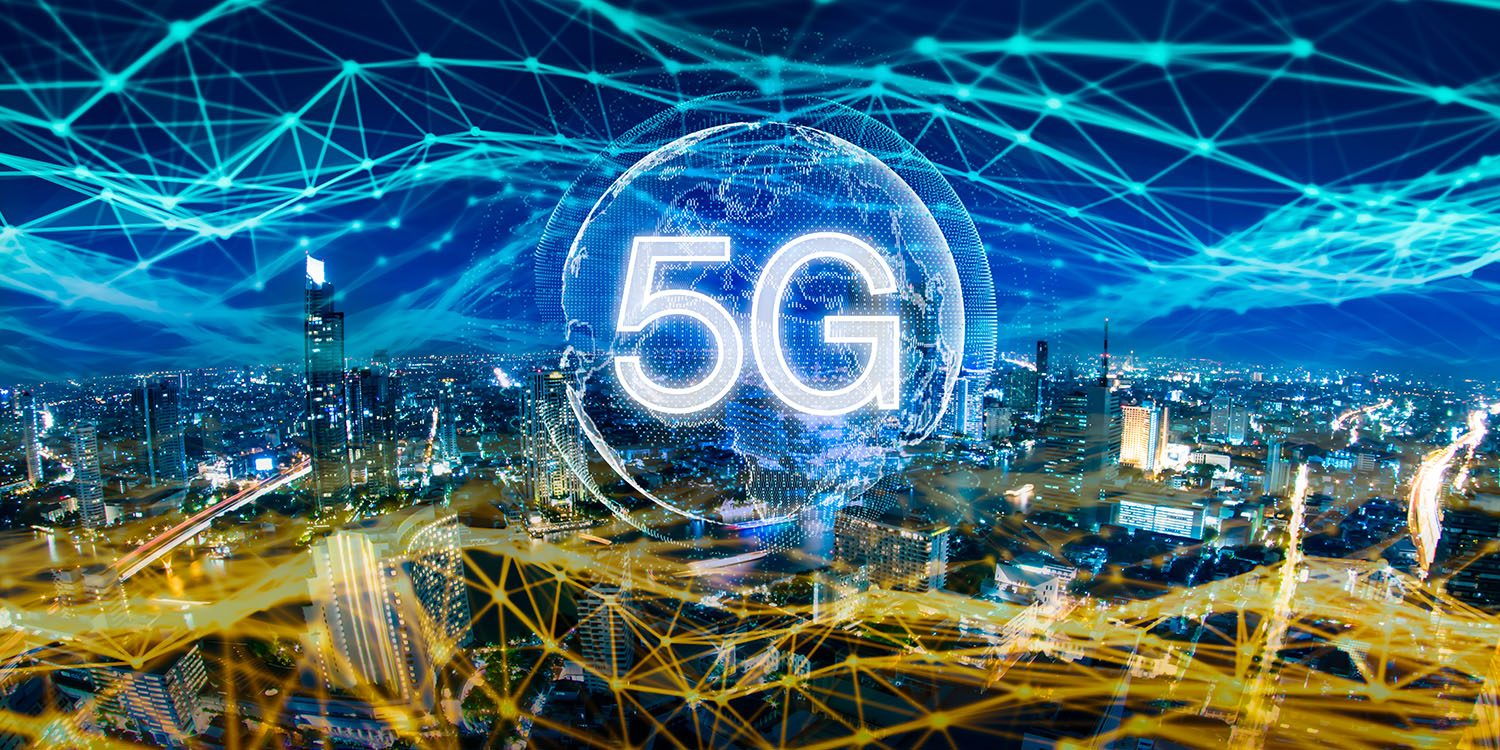
\includegraphics[height=50mm]{Cover/5G}  \end{center} % graficos
 \vspace{5mm}
\centering
\LARGE \textbf{Performance Modelling for \\Social VR Conference Applications in\\Beyond-5G Radio Access Networks}
\\ \vspace{15mm}
%\Large Preparation
%\\ \vspace{15mm}
\Large \textbf{Jo{\~a}o Alberto Janeiro Horta de Morais} \\
\vspace{15mm}
\large Thesis to obtain the Master of Science Degree in
\\ \vspace{2mm}
\LARGE \textbf{Electrical and Computer Engineering}
\\ \vspace{10mm}
\fontsize{14pt}{\baselineskip} \selectfont 
\begin{tabular}{rl}
    Supervisors: & Prof. Ant{\'o}nio Jos{\'e} Castelo Branco Rodrigues \\
    & Prof. Remco Litjens \\
\end{tabular}

\vspace{8mm}
\Large \textbf{Examination Committee}\\ 
\vspace{4mm}
\fontsize{12pt}{\baselineskip} \selectfont 
\begin{tabular}{rl}
    Chairperson: & Prof. Jos{\'e} Eduardo Charters Ribeiro da Cunha Sanguino \\
    Supervisor: & Prof. Ant{\'o}nio Jos{\'e} Castelo Branco Rodrigues \\
    Members of the Committee: & Prof. Ant{\'o}nio Francisco Bucho Cercas \\
\end{tabular}


%\large Prof. Jos{\'e} Eduardo Charters Ribeiro da Cunha Sanguino \\
%\large Chairperson:~Prof.~Jos{\'e}~Eduardo~Charters~Ribeiro~da~Cunha~Sanguino \\
%\large Supervisor: Prof. \\
%\large Co-Supervisor:  Prof .\\
%\large Members of the Committee: \\
\vspace{3mm} %%%%%%%%%%%%%%%%%%5 Add space!

%\Large \textbf{\todaythesis\today} \\
\Large \textbf{February 2021} \\
\let\thepage\relax
\end{flushleft}
\pagebreak


\clearpage
% Since I am using double sided pages, the second page should be white.
% Remember that when delivering the dissertation, IST requires for the cover to appear twice.

\thispagestyle{empty}
\cleardoublepage

\setcounter{page}{1} \pagenumbering{roman}

\baselineskip 18pt % line spacing: -12pt for single spacing
                   %               -18pt for 1 1/2 spacing
                   %               -24pt for double spacingnts}
%\chapter*{Declaration}

I declare that this document is an original work of my own authorship and that 
it fulfils all the requirements of the Code of Conduct and Good Practices of the 
Universidade de Lisboa.
\clearpage
\thispagestyle{empty}
\cleardoublepage


%``C'mon, thousands of hours and I can only pick one quote? Do you think I write stuff like this every Tuesday? I'm choosing as many as I want!'' - Me.


Distorting what Isaac Newton said:

``We can see further by standing upon the shoulders of giants.''
%A thank you to the people that worry about knowledge transfer

Vapnik principle:
``When trying to solve a problem, we should not solve a more difficult problem as an intermediate step.''
%to say thank you for all the advice from my coordinators that helped simplifying the problem when I was trying to solve harder ones as intermediate steps...

Feynman
``We must be careful not to believe things simply because we want them to be true''
It continues to: ``No one can fool you as easily as you can fool yourself''

Alasdair Gray
``Work as if you live in the early days of a better nation''


``Premature optimisation is the root of all evil...''- Donald Knuth - ``... (or at least most of it) in programming.''


``You can never cross the ocean unless you have the courage to lose sight of the shore.'' - Cristóvão Colombo (Christopher Columbus)


``Do things on your own terms, do things in your own time, do things for yourselves, and give everything away.'' - Jacob Collier



\ul{(ideas for quotes. They should be at the bottom)}


\thispagestyle{empty}
\hbox{} \vfill
\begin{flushright}
\small \textit{\textbf{Anyone who has never made a mistake has never tried anything new.}}
\\ \vspace{2mm}  
\scriptsize Albert Einstein
\end{flushright}

\clearpage
\thispagestyle{empty}
\cleardoublepage


%\pdfbookmark{Acknowledgments}{Acknowledgments}
\begin{acknowledgments} 

I would like to thank the Academy, bla bla bla..
\begin{comment}

%To Miguel Amador, for the Thesis Template. Also, more generally, to everyone that strives to transmit knowledge, share their work and allow their findings to be used as a base - to every professor, online lecturer, fellow colleague and everyone curious enough to go extensive lengths while worrying its work can be used by others and built upon.

My professor in Portugal, António Rodrigues, who helped unconditionally when it was needed, sometimes through the \ii{horse's door}, and allowed for a lot of freedom.

Since this marks the end of five years of studying, and I'm not planning on writing another of these any time soon, I should thank who shape my path along the way.
Some professors... Mário Silveirinha, António Topa, ...

And, fortunately, to too many friends to list, with whom I hope not to loose too much contact.



Concrete content contributions to this document:
- Maria for the MCS curves;
- Onno, Yohan, Manolis and Remco for the MIESM figure;
- 
- Remco for some figures;
- Remco and Sjors for reviewing;


HUGE thank you to TNO: invested in hardware necessary to deal with huge amounts of data, letting me using their Cloud for computations, ... and much more



% This is final:

To my advisory team in Hans, Remco and Sjors, for crucial reviews, for more than 50 meetings, more countless emails, and for any physical or virtual interaction. I always learned something. In particular Remco...

To the radio people. To other incredibly nice and no less important 


Niels, ... fortunately, way too many to count! There are more than about 90 people in the department. 

Among these people... Lucia ....

To Lucia (yes, again!), Eduardo, Mike, Dinho, Rosa and others that were the scarce but essential training partners I had during the pandemic.


To my good friends Afonso and Bernardo. For amazing talks that provided the perfect escape after a long day. For accountability with the studies. For the countless rides back and forth when I could not walk. But especially for proving over more than ten years that real friendship does not look at gender, race or social class. Although we are all middle class, white and male... This was a joke. Thanks for always reminding of what fun is.

And to my parents. For always doing their best to give me everything I could need. 


\end{comment}
\end{acknowledgments}
\clearpage
\thispagestyle{empty}
\cleardoublepage
%\begin{abstract}

    One of the most challenging applications targeted by evolving (beyond-)5G technology is virtual reality (VR). Particularly, ‘Social VR’ applications provide a fully immersive experience and sense of togetherness to users residing at different locations. To support such applications the network must deal with enormous traffic demands, while keeping end-to-end latencies low. Moreover, the radio access network must deal with the volatility and vulnerability of mm-wave radio channels, where even small movements of the users may cause line-of-sight blockage, causing severe throughput reductions and hence Quality of Experience (QoE) degradation or even lead to loss of connectivity. In this work we present and validate an integral modelling approach for feasibility assessment and performance optimisation of the radio access network for Social VR applications in indoor office scenarios. Such modelling enables us to determine the performance impact of e.g. ‘natural’ human behaviour, the positions and configurations of the antennas and different resource management strategies. Insights into these issues are a prerequisite for setting up guidelines for network deployment and configuration as well as for the development of (potentially AI/ML-based) methods for dynamic resource management and tuning of radio access parameters to best support Social VR applications.
    
\end{abstract}
%\begin{keywords}
Modelling, Virtual Reality, 5G, Radio Access Networks, Wireless Communications
\end{keywords}
\clearpage
\thispagestyle{empty}
\cleardoublepage
%\begin{resumo}

O objectivo deste trabalho ... (Portugu�s)

\end{resumo}
%\begin{palavraschave}
Modelação, Realidade Virtual, 5G, Redes de Acesso Rádio, Communicações Móveis
\end{palavraschave}
\clearpage
\thispagestyle{empty}
\cleardoublepage
%% This is required for the fancy chapters
\dominitoc
\dominilof
\dominilot

%%%%%%%%%%%%%%%%%%%%%%%%%%%%%%%%%%%%%%%%%%%%%%%%%%%%%%%%%%%%%%%%%%%%%%
% List of contents
%\renewcommand{\baselinestretch}{1}
\pdfbookmark[0]{Index}{index}
\pdfbookmark[1]{Contents}{toc}
\tableofcontents
% \contentsline{chapter}{References}{\pageref{bib}}
\clearpage
\thispagestyle{empty}
\cleardoublepage
%\renewcommand{\baselinestretch}{1.5}
%%%%%%%%%%%%%%%%%%%%%%%%%%%%%%%%%%%%%%%%%%%%%%%%%%%%%%%%%%%%%%%%%%%%%%
% List of figures
\pdfbookmark[1]{List of Figures}{lof}
\listoffigures
\clearpage
\thispagestyle{empty}
\cleardoublepage

%%%%%%%%%%%%%%%%%%%%%%%%%%%%%%%%%%%%%%%%%%%%%%%%%%%%%%%%%%%%%%%%%%%%%%
% List of tables
\pdfbookmark[1]{List of Tables}{lot}
\listoftables
\clearpage
\thispagestyle{empty}
\cleardoublepage

% %%%%%%%%%%%%%%%%%%%%%%%%%%%%%%%%%%%%%%%%%%%%%%%%%%%%%%%%%%%%%%%%%%%%%%
% % List of algorithms
% Requires packages algorithmic, algorithm
% \pdfbookmark[1]{List of Algorithms}{loa}
% \listofalgorithms
% \cleardoublepage
%% %%%%%%%%%%%%%%%%%%%%%%%%%%%%%%%%%%%%%%%%%%%%%%%%%%%%%%%%%%%%%%%%%%%%%%
 % List of acronyms
\pdfbookmark[1]{List of Abbreviations}{loac}

\chapter*{List of Abbreviations}

\acresetall %for resetting acronyms... CHECK THE CAPTIONS NAMES!! MAYBE acs is required there.

% See more at http://staff.science.uva.nl/~polko/HOWTO/LATEX/acronym.html

%these need to be put in order eventually
\begin{acronym}[MU-MIMO] %PUT HERE the longest acronym used for proper alignment
\acro{acro}{Dummy Acronym}

% #
\acro{3GPP}{3rd Generation Partnership Project}
\acro{3G}{3rd Generation}
\acro{4G}{4th Generation}
\acro{5G}{5th Generation}
\acro{5GC}{5th Generation Core}
\acro{5GI}{5G QoS Identifier}

% A

\acro{AAA}{Authentication, Authorisation, and Accounting}
\acro{ACK}{Acknowledgement}
\acro{ADC}{Analog-to-Digital Converter}
\acro{AE}{Antenna Element}
\acro{AFD}{Average Fade Duration}
\acro{AGCH}{Access Grant Channel}
\acro{AI}{Artificial Intelligence}
\acro{AM}{Acknowledged Module}
\acro{AMC}{Adaptive Modulation and Coding}
\acro{AMF}{Access and Mobility Management Function}
\acro{AMPS}{Advanced Mobile Phone System}
\acro{AN}{Access Network}
\acro{ANACOM}{Autoridade Nacional de Comunicações}
\acro{ANSI}{American National Standards Institute}
\acro{AR}{Augmented Reality}
\acro{ARQ}{Automatic Repeat Query}
\acro{AS}{Access Stratum}
\acro{AP}{Access Point}
\acro{API}{Application Programming Interface}
\acro{AuC}{Authentication Centre}
\acro{AWGN}{Additive White Gaussian Noise}



% B
\acro{BB}{Base Band}
\acro{BCCH}{Broadcast Control Channel}
\acro{BCH}{Broadcast Channel}
\acro{BER}{Bit Error Ratio}
\acro{BLER}{Block Error Rate}
\acro{BS}{Base Station}
\acro{BPF}{Band Pass Filter}
\acro{BPSK}{Binary Phase Shift Keying}
\acro{BSC}{Base Station Controller}
\acro{BSS}{Base Station Subsystem}
\acro{BTS}{Base Transceiver Station}
\acro{BU}{Bad Urban}

% C
\acro{CA}{Carrier Aggregation}
\acro{CCCH}{Common Control Channel}
\acro{CCH}{Control Channel}
\acro{CDF}{Cumulative Distribution Function}
\acro{CDMA}{Code Division Multiple Access}
\acro{CENELEC}{Comité Européen de Normalisation Electrotechnique}
\acro{CN}{Core Network}
\acro{CodS}{Coding Scheme}
\acro{CoMP}{Coordinated Multipoint}
\acro{COST}{European Co-operation in the Field of Scientific and Technical Research}
\acro{CP}{Cyclic Prefix}
\acro{CPCH}{Common Packet Channel}
\acro{CPU}{Central Processing Unit}
\acro{CQI}{Channel Quality Indicator}
\acro{CRC}{Cyclic Redundancy Check}
\acro{CS}{Circuit Switch}
\acro{CSI}{Channel State Information}
\acro{CSI-RS}{Channel State Information - Refference Signal}
\acro{CTCH}{Common Traffic Channel}

% D
\acro{D2D}{Device-to-device}
\acro{D-AMPS}{Digital-Advanced Mobile Phone System}
\acro{DAC}{Digital-to-Analog Converter}
\acro{DCCH}{Dedicated Control Channel}
\acro{DCH}{Dedicated Channel}
\acro{DECT}{Digital Enhanced Cordless Telecommunications}
\acro{DL}{Downlink}
\acro{DN}{Data Network}
\acro{DNN}{Deep Neural Network}
\acro{DPCCH}{Dedicated Physical Control Channel}
\acro{DPDCH}{Dedicated Physical Data Channel}
\acro{DQPSK}{Differential Quadrature Phase Shift Keying}
\acro{DRB}{Data Radio Bearer}
\acro{DSCH}{Dedicated Shared Channel}
\acro{DTCH}{Dedicated Traffic Channel}

% E
\acro{EBF}{Explicit Beamforming}
\acro{EGC}{Equal Gain Combining}
\acro{EGDE}{Enhanced Data rates for GSM Evolution}
\acro{EHD}{Environmental Health Division}
\acro{EHF}{Extremely High Frequency}
\acro{EIRP}{Equivalent Isotropic Radiated Power}
\acro{eMBB}{extreme Mobile Broadband}
\acro{eNB}{evolved Node B}
\acro{EPC}{Evolved Packet Core}
\acro{ERPd}{Effective Radiated Power by half wavelength dipole}
\acro{ESN}{Echo State Network}
\acro{E-UTRA}{Evolved-UMTS Terrestrial Radio Access}
\acro{E-UTRAN}{Evolved-UMTS Terrestrial Radio Access Network}
\acro{EXP/PF}{Exponential/Proportional Fair}

% F
\acro{FACCH}{Fast Associated Control Channel}
\acro{FACH}{Forward Access Channel}
\acro{FCCH}{Frequency Correction Channel}
\acro{FDD}{Frequency Division Duplex}
\acro{FDM}{Frequency-Division Multiplexing}
\acro{FDMA}{Frequency-Division Multiple Access}
\acro{FEC}{Foward Error Correction}
\acro{FIFO}{First In First Out}
\acro{FM}{Frequency Modulation}
\acro{FNBW}{First Null Beam Width}
\acro{FOV}{Field Of View}
\acro{FR}{Frequency Range}
\acro{FPS}{Frames Per second}
\acro{FTP}{File Transfer Protocol}
\acro{FWA}{Fixed Wireless Access}


% G
\acro{GB}{GigaBytes}
\acro{GBR}{Guaranteed Bit Rate}
\acro{GGSN}{Gateway GPRS Support Node}
\acro{GMSK}{Gaussian Minimum Shift Keying}
\acro{gNB}{Next Generation Node B}
\acro{GoB}{Grid of Beams}
\acro{GoP}{Group of Pictures}
\acro{GoS}{Grade of Service}
\acro{GPRS}{General Packet Radio System}
\acro{GPT-U}{GPRS Tunneling Protocol User plane}
\acro{GSM}{Global System for Mobile Communications}

% H
\acro{HARQ}{Hybrid Automatic Repeat Request}
\acro{HEVC}{High Efficiency Video Coding}
\acro{HF}{High Frequency}
\acro{HLR}{Home Location Register}
\acro{HMD}{Head Mounted Display}
\acro{HO}{Handover}
\acro{HPBW}{Half-Power Beam Width}
\acro{HSCSD}{High Speed Circuit Switched Data}
\acro{HSDPA}{High-Speed Downlink Packet Access}
\acro{HSPA}{High-Speed Packet Access}
\acro{HSS}{Home Subscriber Server}
\acro{HSUPA}{High-Speed Uplink Packet Access}
\acro{HT}{Hilly Terrain}
\acro{HTTP}{Hypertext Transfer Protocol}

% I
\acro{IBF}{Implicit Beamforming}
\acro{ICIC}{Inter-Cell Interference Coordination}
\acro{ICNIRP}{International Commission on Non-Ionising Radiation Protection}
\acro{IEEE}{Institute of Electrical and Electronics Engineers}
\acro{IF}{Intermediate Frequency}
\acro{IMS}{IP Multimedia Subsystem}
\acro{IP}{Internet Protocol}
\acro{IQ}{In-phase and Quadrature}
\acro{IRPA}{International Radiation Protection Association}
\acro{IS-94}{Interim Standard 94}
\acro{ISDN}{Integrated Services Digital Network}
\acro{ISI}{Inter-Symbol Interference}
\acro{ITU}{International Telecommunications Union}
\acro{ITU-R}{International Telecommunications Union – Radio sector}

% J

% K
\acro{KPI}{Key Performance Indicator}

% L
\acro{L1}{Layer 1}
\acro{L2}{Layer 2}
\acro{L3}{Layer 3}
\acro{L4}{Layer 4}
\acro{L5}{Layer 5}
\acro{LAN}{Local Area Network}
\acro{LBT}{Listen-before-talk}
\acro{LCR}{Level Crossing Rate}
\acro{LF}{Low Frequency}
\acro{LIFO}{Last In First Out}
\acro{LLC}{Link Layer Control}
\acro{LMS}{Least Mean Squares}
\acro{LoS}{Line-of-Sight}
\acro{LTE}{Long-Term Evolution}

% M
\acro{MAC}{Medium Access Control}
\acro{MCS}{Modulation and Coding Scheme}
\acro{MCU}{Multi-point Control Unit}
\acro{MF}{Medium Frequency}
\acro{MIMO}{Multiple-Input Multiple-Output}
\acro{MIESM}{Mutual Information Effective SINR Mapping}
\acro{M-LWDF}{Maximum-Largest Weighted Delay First}
\acro{MME}{Mobility Management Entity}
\acro{MMSE}{Minimum Mean-Square Error}
\acro{mMTC}{massive Machine-Type Communications}
\acro{mmWave}{Millimetre Wave}
\acro{ML}{Machine Learning}
\acro{MR}{Maximum Ratio}
\acro{MRC}{Maximum Ratio Combining}
\acro{MRT}{Maximum Ratio Trasmission}
\acro{MSC}{Mobile Switching Centre}
\acro{MTP}{Motion-to-photon}
\acro{MU-MIMO}{Multi-user MIMO}

% N
\acro{NAMTS}{NEC Advance Mobile Telephone System}
\acro{NAS}{Non-Access Stratum}
\acro{NB}{Node B}
\acro{NEC}{Nippon Electric Company}
\acro{NLoS}{Non-Line-of-Sight}
\acro{NMT}{Nordic Mobile Telephone}
\acro{NN}{Neural Network}
\acro{nGBR}{Non-Guaranteed Bit Rate}
\acro{NG}{Next Generation}
\acro{ng-eNB}{Next Generation evolved Node B}
\acro{NG-AP}{Next Generation Application Protocol}
\acro{NG-RAN}{Next Generation Radio Access Network}
\acro{NR}{New Radio}





% O
\acro{OFDM}{Orthogonal Frequency Division Multiplexing}
\acro{OFDMA}{Orthogonal Frequency Division Multiple Access}
\acro{OLLA}{Outer Loop Link Adaptation}
\acro{OSI}{Open Systems Interconnection}
\acro{OVSF}{Orthogonal Variable Spreading Factor}

% P
\acro{PAPR}{Peak-to-Average-Power Ratio}
\acro{PCCH}{Paging Control Channel}
\acro{P-CCPCH}{Primary Common Control Physical Channel}
\acro{PCH}{Paging Channel}
\acro{PCPCH}{Physical Common Packet Channel}
\acro{PCRF}{Policy and Charging Rules Function}
\acro{PCU}{Packet Control Unit}
\acro{PDA}{Personal Digital Assistant}
\acro{PDC}{Personal Digital Cellular}
\acro{PDCP}{Packet Data Convergence Protocol}
\acro{PDF}{Probability Density Function}
\acro{PDN}{Packet Data Network}
\acro{PDP}{Power Delay Profile}
\acro{PDSCH}{Physical Downlink Shared Channel}
\acro{PDSN}{Packet Data Serving Node}
\acro{PDTCH}{Packet Data Traffic Channel}
\acro{PDU}{Protocol Data Unit}
\acro{PER}{Packet Error Ratio}
\acro{PF}{Proportional Fair}
\acro{P-GW}{PDN Gateway}
\acro{PH}{Power Headroom}
\acro{PHY}{Physical}
\acro{PLMN}{Public Land Mobile Network}
\acro{PN}{Packet Network}
\acro{PRACH}{Physical Random Access Channel}
\acro{PRB}{Physical Resource Block}
\acro{PS}{Packet Switch}
\acro{PSC}{Pure Selection Combining}
\acro{PSK}{Phase Shift Keying}
\acro{PSTN}{Public Switch Telecommunications Network}

% Q
\acro{QAM}{Quadrature Amplitude Modulation}
\acro{QCI}{Quality Channel Indicator}
\acro{QPSK}{Quadrature Phase Shift Keying}
\acro{QoE}{Quality of Experience}
\acro{QoS}{Quality of Service}

% R
\acro{R2000}{Radiocom 2000}
\acro{RA}{Rural Area}
\acro{RACH}{Random Access Channel}
\acro{RADAR}{RAdio Detection And Ranging}
\acro{RAM}{Random Access Memory}
\acro{RAN}{Radio Access Network}
\acro{RAT}{Radio Access Technology}
\acro{RB}{Resource Block}
\acro{RBG}{Resource Blocks Group}
\acro{RE}{Resource Element}
\acro{Rel15}{Release 15}
\acro{Rel16}{Release 16}
\acro{RF}{Radio Frequency}
\acro{RGB}{Red Green Blue}
\acro{RLC}{Radio Link Control}
\acro{RL}{Reinforcement Learning}
\acro{RLS}{Recursive Least Squares}
\acro{RM}{Resource Management}
\acro{RMTS}{Radio Mobile Telephone System}
\acro{RNC}{Radio Network Controller}
\acro{RNN}{Recurrent Neural Network}
\acro{RNS}{Radio Network Subsystem}
\acro{ROHC}{Robust Header Compression}
\acro{RR}{Radio Resource}
\acro{RRC}{Radio Resource Control}
\acro{RRM}{Radio Resource Management}
\acro{RRMM}{Radio Resource Management Mechanism}
\acro{RSS}{Received Signal Strength}
\acro{RTT}{Round Trip Time}
\acro{Rx}{Receiver}
\acro{RX}{Receiver}
\acro{RZF}{Regularised Zero Forcing}







% S
\acro{SACCH}{Slow Associated Control Channel}
\acro{SAE}{System Architecture Evolution}
\acro{SAR}{Specific Absorption Rate}
\acro{SAT}{Satisfiable}
\acro{S-CCPCH}{Secondary Common Control Physical Channel}
\acro{SC-FDMA}{Single Carrier Frequency Division Multiple Access}
\acro{SCH}{Synchronisation Channel}
\acro{SCTP}{Stream Control Transmission Protocol}
\acro{SDAP}{Service Data Adaptation Protocol}
\acro{SDCCH}{Stand-alone Dedicated Control Channel}
\acro{SDF}{Service Data Flow}
\acro{SDU}{Service Data Unit}
\acro{SDMA}{Space Division Multiple Access}
\acro{SE}{Spectral Efficiency}
\acro{SF}{Spreading Factor}
\acro{SGSN}{Serving GPRS Support Node}
\acro{S-GW}{Serving Gateway}
\acro{SHF}{Super High Frequency}
\acro{SIM}{Subscriber Identity Module}
\acro{SINR}{Signal-to-Interference-plus-Noise Ratio}
\acro{SLL}{Side Lobe Level}
\acro{SLS}{System-Level Simulator}
\acro{SMF}{Session Management Function}
\acro{SMS}{Short Message Service}
\acro{SNR}{Signal to Noise Ratio}
\acro{SRB}{Signalling Radio Bearer}
\acro{SRS}{Sounding Reference Signal}
\acro{SS7}{Signalling System \#7}

% T
\acro{TACS}{Total Access Communication System}
\acro{TB}{Transport Block}
\acro{TBS}{Transport Block Size}
\acro{TCH}{Traffic Channels}
\acro{TCP}{Transmission Control Protocol}
\acro{TDD}{Time Division Duplex}
\acro{TDM}{Time Division Multiplexing}
\acro{TDMA}{Time Division Multiple Access}
\acro{TETRA}{Terrestrial Trunked Radio}
\acro{TM}{Transparent Mode}
\acro{TSG}{Technical Specification Group}
\acro{TS}{Technical Speficiation}
\acro{TSC}{Threshold Selection Combining}
\acro{TR}{Technical Report}
\acro{TTI}{Transmission Time Interval}
\acro{TU}{Typical Urban}
\acro{TV}{Television}
\acro{Tx}{Transmitter}
\acro{TX}{Transmitter}

% U
\acro{UDP}{User Datagram Protocol}
\acro{UE}{User Equipment}
\acro{UHF}{Ultra High Frequency}
\acro{UL}{Uplink}
\acro{ULA}{Uniform Linear Array}
\acro{UM}{Unackowledged Mode}
\acro{UMTS}{Universal Mobile Telecommunications System}
\acro{UP}{User Plane}
\acro{UPF}{User Plane Function}
\acro{URA}{Uniform Rectangular Array}
\acro{URLLC}{Ultra-reliable Low-Latency Communications}
\acro{UTD}{Uniform Theory of Diffraction}
\acro{UTRAN}{UMTS Terrestrial Radio Access Network}

% V
\acro{V2I}{Vehicle-to-Infrastructure}
\acro{V2V}{Vehicle-to-Vehicle}
\acro{VHF}{Very High Frequency}
\acro{VLF}{Very Low Frequency}
\acro{VLR}{Visitors Location Register}
\acro{VoIP}{Voice over IP}
\acro{VR}{Virtual Reality}

% X
\acro{XR}{Extended Reality}
% Y

% W
\acro{WG}{Working Group}
\acro{WHO}{World Health Organisation}
\acro{WLAN}{Wireless LAN}

% Z
\acro{ZF}{Zero Forcing}


\end{acronym}

\clearpage
\thispagestyle{empty}
%\cleardoublepage



 %Uncomment clear double page inside this .tex
%%%%%%%%%%%%%%%%%%%%%%%%%%%%%%%%%%%%%%%%%%%%%%%%%%%%%%%%%%%%%%%%%%%%%%%
% List of symbols
\pdfbookmark[1]{List of Symbols}{los}



% IF there's time:
% MIGRATE THIS LIST OF SYMBOLS TO \newsym based! When the thesis is written, so we know where the first
% instance of the symbol is.

% \newsym{<description>}{<symbol>}
% from: https://personal.utdallas.edu/~kxh060100/symlist.pdf

% ONLY DO THIS if the 'dots between description and page number
% can be removed.

% It would also be nice to have different headings.




% RULE 1:
% NOTE ON THE MATHEMATICAL SYMBOLS TO USE
% As epsilon, use the first variant!

%\varepsilon for ε and \epsilon for ϵ
%\theta for θ and \vartheta for ϑ
%\pi for π and \varpi for or ϖ
%\rho for ρ and \varrho for ϱ
%\sigma for σ and \varsigma for ς
%\varphi for φ and \phi for ϕ

% Start of the list of Symbols
% have 3 lists: Sets, greek letters, normal letters


% RULE 2:
% All symbols are italic (subscripts and superscripts don't need to be)
% except matrices 

% \tab is given in the tabto package
\newcommand\mytab{\tab \hspace{-5cm}}

% If the box is not visually overfull, ignore the warning
% it has to do with the huge tab.



\chapter*{List of Symbols} \todo{should this be called nomenclature instead?}
(not perfectly alphabetically ordered \ii{yet})

\subsubsection*{Latin alphabet}

% A

% B
$B$ \mytab bandwidth \\
$BLER_0$ \mytab target \acs{BLER} \\



% C

% D

% E
$E_b$ \mytab energy per bit \\

% F

% G

% H
$\bm{H}_{bmp}$ \mytab channel matrix between BS $b$ and UE $m$ in BSs polarisation $p$\\

% I
% J
$j$ \mytab imaginary unit $\left(j = \sqrt{-1}\right)$\\


% K
$k_B$ \mytab Boltzmann constant\\

% L for lengths, and latencies -> this will change
$L_{max}$ \mytab maximum latency for the radio link \\
$L_\text{sch}$  \mytab length of scheduling information update period \\
$L_\text{csi}$  \mytab length of \acs{CSI} update period \\
$L_\text{slot}$ \mytab length of slot period \\
$L_\text{TB}$ \mytab length of a transport block, in bits \\

% M

% N (for numbers of something, mainly)
$N_0$ \mytab noise power spectral density \\
$N_r$ \mytab number of receive antennas \\
$N_t$ \mytab number of transmit antennas \\
$N_{phy}$ \mytab number of physical users \\
$N_{vir}$ \mytab number of virtual users \\
$N_\text{CSI Beams}$ \mytab number of beams with CSI-RS, per polarisation \\
$N_\text{BS}$ \mytab number of \acsp{BS} \\
$N_\text{UE}$ \mytab number of \acsp{UE} \\
$N_\text{symb}^\text{PRB}$ \mytab number of symbols per PRB \\
$N_\text{bits}^\text{symb}$ \mytab number of bits per symbol \\
$N_\text{info bits}^\text{symb}$ \mytab number of information bits per symbol \\
$N_\text{bits}^\text{slot}$ \mytab number of bits per slot \\
$N_\text{req PRB}$ \mytab number of requested PRBs by a UE for an UL transmission \\
$N_\text{TB}^\text{slot}$ \mytab number of transport blocks per slot \\
$N_{bml}^\text{PRB}$ \mytab number of PRBs scheduled for a transmission \\
${ }$ \mytab between BS $b$ and UE $m$ in layer $l$ \\
$NF_r$ \mytab noise figure at the receiver \\
$N_x$ \mytab number of antennas along the x-dimension\\
$N_y$ \mytab number of antennas along the y-dimension\\
$NF_\text{BS}$ \mytab BS noise figure \\
$NF_\text{UE}$ \mytab UE noise figure\\

% O

% P (used for powers)
$P_n$ \mytab noise power \\
$P_r$ \mytab received power \\
$P_s$ \mytab received signal power \\
$P_t$ \mytab transmit power \\
$P_t^\text{UE}$ \mytab maximum transmit power per UE\\
$P_t^\text{BS}$ \mytab maximum transmit power per BS \\
$P_{bml}^\text{BS}$ \mytab transmit power at the BS for a link between BS $b$ and UE $m$ in layer $l$ \\
$P_{bml}^\text{UE}$ \mytab transmit power at the UE for a link between BS $b$ and  UE $m$ in layer $l$ \\
$P_\text{IntraCI}$ \mytab interference power from intra-cell interference sources \\
$P_\text{InterCI}$ \mytab interference power from inter-cell interference sources \\
$P_\text{ILI}$ \mytab interference power from inter-layer interference \\
${ }$ \mytab (applicable when there is a multi-layer transmission) \\
$P_\text{PRB}$ \mytab transmit power per PRB \\

% Q
$Q_m$ \mytab modulation order \\
$Q_{P-I}$ \mytab P-frame to I-frame ratio \\

% R
$R_b$ \mytab bit rate \\
$\hat{R}_b$ \mytab estimated bit rate \\
$R_c$ \mytab code rate \\
$\overline{R}_{DL}$ \mytab average application information rate in the \ac{DL}\\

% S
$s_\text{TDD}$ \mytab TDD split \\
$SINR_\text{eff}$ \mytab effective SINR, i.e. aggregated over all scheduled PRBs \\
$SINR_i$ \mytab SINR of the i-th PRB \\
$S_t$ \mytab power spectral density at transmission\\
$S_I$ \mytab size of I frame\\
$S_P$ \mytab size of P frame\\

% T for periods [s] and Temperatures
$T_\text{slot}$  \mytab slot duration \\
$T$ \mytab noise temperature\\

% U

% V

% X

% Y

% W
$\bm{w}$ \mytab vector of beamforming weights \\
$\bm{w}_{\phi, \theta}$ \mytab vector of beamforming weights from a GoB with direction $(\phi, \theta)$ \\
$\bm{w}_{i,j}$ \mytab vector of beamforming weights from a GoB with grid indices $(i,j)$\\

% Z

%\vspace{1cm}

\subsubsection*{Greek alphabet}

% Alpha (Α α)
$\alpha_P$ \mytab power compensation factor for UL power control\\

% Beta (Β β)

% Gamma (Γ γ)
$\gamma_{OLLA}$ \mytab step size for OLLA parameter ($\Delta_{OLLA}$) update\\

% Delta (Δ δ)
$\Delta_{OLLA}$ \mytab outer loop link adaptation step\\

% Ε ε
% Ζ ζ
% Η η
% Θ θ
% Ι ι
% Κ κ
% Λ λ
% Μ μ
% Ν ν
% Ξ ξ
% Ο ο
% Π π
% Ρ ρ
$\rho$ \mytab number of bits per symbol, used in SINR mapping algorithm (MIESM)\\

% Σ σ/ς
% Tau (Τ τ)  - used for delays
$\tau_\text{CSI}$   \mytab \acsp{CSI} delay in number of \acsp{TTI} \\
% Υ υ
% Φ φ
% Χ χ
% Ψ ψ
% Ω ω







\subsubsection*{Sets:}

$\mathbb{N}$ \mytab set of natural numbers \\
$\mathbb{N}_0$ \mytab set of natural numbers including zero\\





\subsubsection*{Other nomenclature}


$\bm{A}$ \mytab matrix\\

$\bm{a}$ \mytab column vector\\

$|\bm{a}|$ \mytab euclidean norm of vector $\bm{a}$\\

$\bm{A}^\text{T}$ \mytab transpose of $\bm{A}$\\
$\bm{A}^\text{H}$ \mytab Hermitian of $\bm{A}$, also know as the transpose conjugate of $\bm{A}$\\

% $\ceil{a}{b}$ \mytab Ceil $a$ to $b$ decimal places, i.e. round $a$ to the next $10^-b$. 
$\ceil{a}$ \mytab ceil $a$, i.e. round up $a$ to the nearest integer\\

$\floor{\cdot}$ \mytab floor $a$, i.e. round down $a$ to the nearest integer \\


% $A_\text{[dB]}$ \mytab the quantity A is expressed in dB.\\






\clearpage
\thispagestyle{empty}


\cleardoublepage
% Pages number is starting now with arabic style... until now it was on roman mode
\pagenumbering{arabic} \setcounter{page}{1}
\baselineskip 18pt

%\setcounter{page}{1} \pagenumbering{Alph}

% Add PDF bookmark 
\pdfbookmark[0]{Title}{Title}

\thispagestyle{empty}
\begin{flushleft} ~\\ \vspace{-12mm} \hspace{-12mm}  
\includegraphics[width=50mm]{Cover/istnewlogo} 
\vspace{10mm}
%~\\ \vspace{50mm} % gr�ficos
\\ \begin{center} 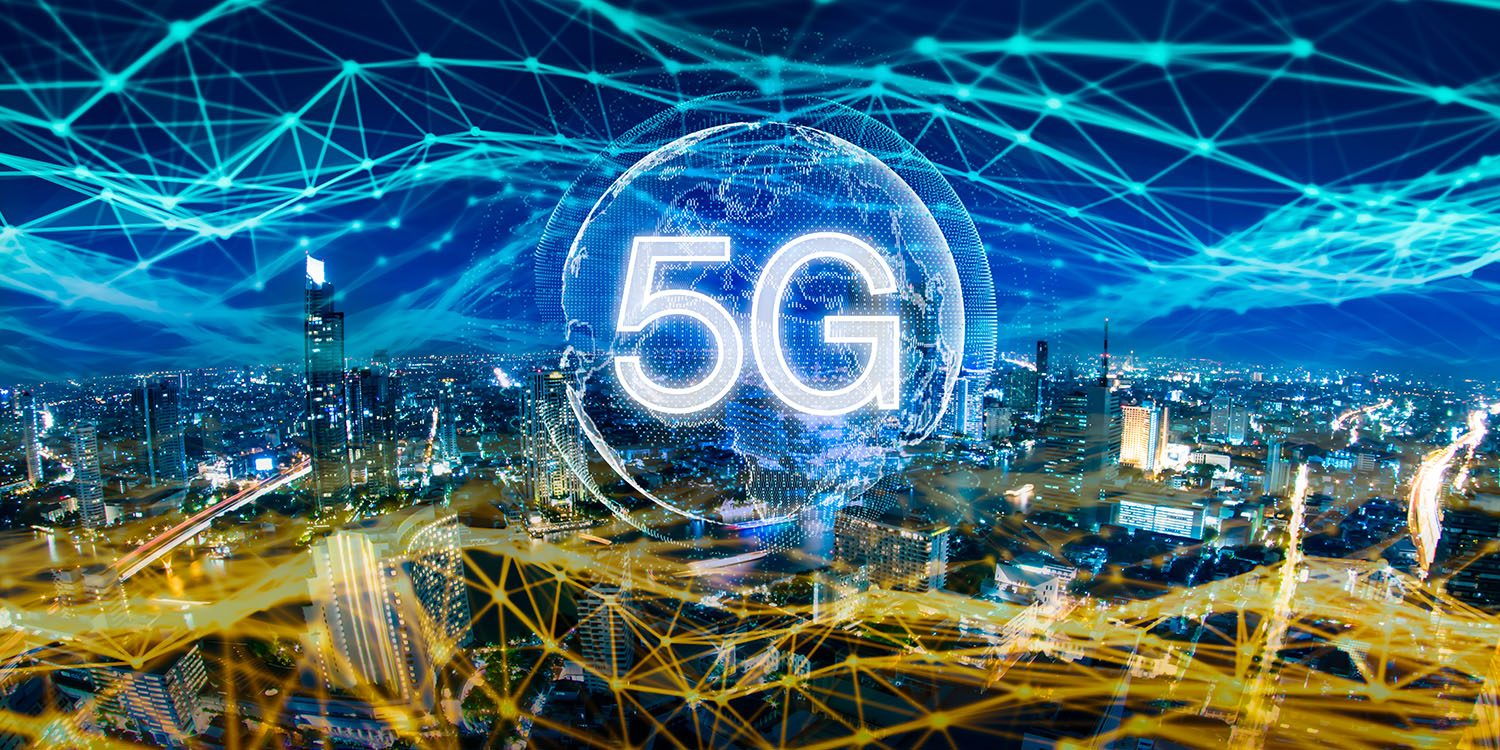
\includegraphics[height=50mm]{Cover/5G}  \end{center} % graficos
 \vspace{5mm}
\centering
\LARGE \textbf{Performance Modelling for \\Social VR Conference Applications in\\Beyond-5G Radio Access Networks}
\\ \vspace{15mm}
%\Large Preparation
%\\ \vspace{15mm}
\Large \textbf{Jo{\~a}o Alberto Janeiro Horta de Morais} \\
\vspace{15mm}
\large Thesis to obtain the Master of Science Degree in
\\ \vspace{2mm}
\LARGE \textbf{Electrical and Computer Engineering}
\\ \vspace{10mm}
\fontsize{14pt}{\baselineskip} \selectfont 
\begin{tabular}{rl}
    Supervisors: & Prof. Ant{\'o}nio Jos{\'e} Castelo Branco Rodrigues \\
    & Prof. Remco Litjens \\
\end{tabular}

\vspace{8mm}
\Large \textbf{Examination Committee}\\ 
\vspace{4mm}
\fontsize{12pt}{\baselineskip} \selectfont 
\begin{tabular}{rl}
    Chairperson: & Prof. Jos{\'e} Eduardo Charters Ribeiro da Cunha Sanguino \\
    Supervisor: & Prof. Ant{\'o}nio Jos{\'e} Castelo Branco Rodrigues \\
    Members of the Committee: & Prof. Ant{\'o}nio Francisco Bucho Cercas \\
\end{tabular}


%\large Prof. Jos{\'e} Eduardo Charters Ribeiro da Cunha Sanguino \\
%\large Chairperson:~Prof.~Jos{\'e}~Eduardo~Charters~Ribeiro~da~Cunha~Sanguino \\
%\large Supervisor: Prof. \\
%\large Co-Supervisor:  Prof .\\
%\large Members of the Committee: \\
\vspace{3mm} %%%%%%%%%%%%%%%%%%5 Add space!

%\Large \textbf{\todaythesis\today} \\
\Large \textbf{February 2021} \\
\let\thepage\relax
\end{flushleft}
\pagebreak


\clearpage
% Since I am using double sided pages, the second page should be white.
% Remember that when delivering the dissertation, IST requires for the cover to appear twice.

\thispagestyle{empty}
\cleardoublepage

\setcounter{page}{1} \pagenumbering{roman}

\baselineskip 18pt % line spacing: -12pt for single spacing
                   %               -18pt for 1 1/2 spacing
                   %               -24pt for double spacingnts}
\chapter*{Declaration}

I declare that this document is an original work of my own authorship and that 
it fulfils all the requirements of the Code of Conduct and Good Practices of the 
Universidade de Lisboa.
\clearpage
\thispagestyle{empty}
\cleardoublepage

   
\begin{center}
    \LARGE \bb{Foreword}
\end{center}

\vspace{1cm}

The research presented in this document was conducted in TNO as part of a project called ‘Empowered Edge’, in the first year of a large research programme on Social-Extended Reality. Naturally, the research will continue and one of the main concerns throughout of this project has been guaranteeing flexibility 


to use this simulator and several directions described in the future work section will be pursued.


This thesis




% the direction this is taking...

% this allowed one internship and 2 MSc thesis

% working on this project also facilitated the process of creating two patents for other projects within TNO.
``C'mon, thousands of hours and I can only pick one quote? Do you think I write stuff like this every Tuesday? I'm choosing as many as I want!'' - Me.


Distorting what Isaac Newton said:

``We can see further by standing upon the shoulders of giants.''
%A thank you to the people that worry about knowledge transfer

Vapnik principle:
``When trying to solve a problem, we should not solve a more difficult problem as an intermediate step.''
%to say thank you for all the advice from my coordinators that helped simplifying the problem when I was trying to solve harder ones as intermediate steps...

Feynman
``We must be careful not to believe things simply because we want them to be true''
It continues to: ``No one can fool you as easily as you can fool yourself''

Alasdair Gray
``Work as if you live in the early days of a better nation''


``Premature optimisation is the root of all evil...''- Donald Knuth - ``... (or at least most of it) in programming.''


``You can never cross the ocean unless you have the courage to lose sight of the shore.'' - Cristóvão Colombo (Christopher Columbus)


``Do things on your own terms, do things in your own time, do things for yourselves, and give everything away.'' - Jacob Collier



\ul{(ideas for quotes. They should be at the bottom)}


\thispagestyle{empty}
\hbox{} \vfill
\begin{flushright}
\small \textit{\textbf{Anyone who has never made a mistake has never tried anything new.}}
\\ \vspace{2mm}  
\scriptsize Albert Einstein
\end{flushright}

\clearpage
\thispagestyle{empty}
\cleardoublepage


\pdfbookmark{Acknowledgments}{Acknowledgments}
\begin{acknowledgments} 

I would like to thank the Academy, bla bla bla..
\begin{comment}

%To Miguel Amador, for the Thesis Template. Also, more generally, to everyone that strives to transmit knowledge, share their work and allow their findings to be used as a base - to every professor, online lecturer, fellow colleague and everyone curious enough to go extensive lengths while worrying its work can be used by others and built upon.

My professor in Portugal, António Rodrigues, who helped unconditionally when it was needed, sometimes through the \ii{horse's door}, and allowed for a lot of freedom.

Since this marks the end of five years of studying, and I'm not planning on writing another of these any time soon, I should thank who shape my path along the way.
Some professors... Mário Silveirinha, António Topa, ...

And, fortunately, to too many friends to list, with whom I hope not to loose too much contact.



Concrete content contributions to this document:
- Maria for the MCS curves;
- Onno, Yohan, Manolis and Remco for the MIESM figure;
- 
- Remco for some figures;
- Remco and Sjors for reviewing;


HUGE thank you to TNO: invested in hardware necessary to deal with huge amounts of data, letting me using their Cloud for computations, ... and much more



% This is final:

To my advisory team in Hans, Remco and Sjors, for crucial reviews, for more than 50 meetings, more countless emails, and for any physical or virtual interaction. I always learned something. In particular Remco...

To the radio people. To other incredibly nice and no less important 


Niels, ... fortunately, way too many to count! There are more than about 90 people in the department. 

Among these people... Lucia ....

To Lucia (yes, again!), Eduardo, Mike, Dinho, Rosa and others that were the scarce but essential training partners I had during the pandemic.


To my good friends Afonso and Bernardo. For amazing talks that provided the perfect escape after a long day. For accountability with the studies. For the countless rides back and forth when I could not walk. But especially for proving over more than ten years that real friendship does not look at gender, race or social class. Although we are all middle class, white and male... This was a joke. Thanks for always reminding of what fun is.

And to my parents. For always doing their best to give me everything I could need. 


\end{comment}
\end{acknowledgments}
\clearpage
\thispagestyle{empty}
\cleardoublepage
\begin{abstract}

    One of the most challenging applications targeted by evolving (beyond-)5G technology is virtual reality (VR). Particularly, ‘Social VR’ applications provide a fully immersive experience and sense of togetherness to users residing at different locations. To support such applications the network must deal with enormous traffic demands, while keeping end-to-end latencies low. Moreover, the radio access network must deal with the volatility and vulnerability of mm-wave radio channels, where even small movements of the users may cause line-of-sight blockage, causing severe throughput reductions and hence Quality of Experience (QoE) degradation or even lead to loss of connectivity. In this work we present and validate an integral modelling approach for feasibility assessment and performance optimisation of the radio access network for Social VR applications in indoor office scenarios. Such modelling enables us to determine the performance impact of e.g. ‘natural’ human behaviour, the positions and configurations of the antennas and different resource management strategies. Insights into these issues are a prerequisite for setting up guidelines for network deployment and configuration as well as for the development of (potentially AI/ML-based) methods for dynamic resource management and tuning of radio access parameters to best support Social VR applications.
    
\end{abstract}
\begin{keywords}
Modelling, Virtual Reality, 5G, Radio Access Networks, Wireless Communications
\end{keywords}
\clearpage
\thispagestyle{empty}
\cleardoublepage
\begin{resumo}

O objectivo deste trabalho ... (Portugu�s)

\end{resumo}            
\begin{palavraschave}
Modelação, Realidade Virtual, 5G, Redes de Acesso Rádio, Communicações Móveis
\end{palavraschave}
\clearpage
\thispagestyle{empty}
\cleardoublepage  
% This is required for the fancy chapters
\dominitoc
\dominilof
\dominilot

%%%%%%%%%%%%%%%%%%%%%%%%%%%%%%%%%%%%%%%%%%%%%%%%%%%%%%%%%%%%%%%%%%%%%%
% List of contents
%\renewcommand{\baselinestretch}{1}
\pdfbookmark[0]{Index}{index}
\pdfbookmark[1]{Contents}{toc}
\tableofcontents
% \contentsline{chapter}{References}{\pageref{bib}}
\clearpage
\thispagestyle{empty}
\cleardoublepage
%\renewcommand{\baselinestretch}{1.5}
%%%%%%%%%%%%%%%%%%%%%%%%%%%%%%%%%%%%%%%%%%%%%%%%%%%%%%%%%%%%%%%%%%%%%%
% List of figures
\pdfbookmark[1]{List of Figures}{lof}
\listoffigures
\clearpage
\thispagestyle{empty}
\cleardoublepage

%%%%%%%%%%%%%%%%%%%%%%%%%%%%%%%%%%%%%%%%%%%%%%%%%%%%%%%%%%%%%%%%%%%%%%
% List of tables
\pdfbookmark[1]{List of Tables}{lot}
\listoftables
\clearpage
\thispagestyle{empty}
\cleardoublepage

% %%%%%%%%%%%%%%%%%%%%%%%%%%%%%%%%%%%%%%%%%%%%%%%%%%%%%%%%%%%%%%%%%%%%%%
% % List of algorithms
% Requires packages algorithmic, algorithm
% \pdfbookmark[1]{List of Algorithms}{loa}
% \listofalgorithms
% \cleardoublepage
% %%%%%%%%%%%%%%%%%%%%%%%%%%%%%%%%%%%%%%%%%%%%%%%%%%%%%%%%%%%%%%%%%%%%%%
 % List of acronyms
\pdfbookmark[1]{List of Abbreviations}{loac}

\chapter*{List of Abbreviations}

\acresetall %for resetting acronyms... CHECK THE CAPTIONS NAMES!! MAYBE acs is required there.

% See more at http://staff.science.uva.nl/~polko/HOWTO/LATEX/acronym.html

%these need to be put in order eventually
\begin{acronym}[MU-MIMO] %PUT HERE the longest acronym used for proper alignment
\acro{acro}{Dummy Acronym}

% #
\acro{3GPP}{3rd Generation Partnership Project}
\acro{3G}{3rd Generation}
\acro{4G}{4th Generation}
\acro{5G}{5th Generation}
\acro{5GC}{5th Generation Core}
\acro{5GI}{5G QoS Identifier}

% A

\acro{AAA}{Authentication, Authorisation, and Accounting}
\acro{ACK}{Acknowledgement}
\acro{ADC}{Analog-to-Digital Converter}
\acro{AE}{Antenna Element}
\acro{AFD}{Average Fade Duration}
\acro{AGCH}{Access Grant Channel}
\acro{AI}{Artificial Intelligence}
\acro{AM}{Acknowledged Module}
\acro{AMC}{Adaptive Modulation and Coding}
\acro{AMF}{Access and Mobility Management Function}
\acro{AMPS}{Advanced Mobile Phone System}
\acro{AN}{Access Network}
\acro{ANACOM}{Autoridade Nacional de Comunicações}
\acro{ANSI}{American National Standards Institute}
\acro{AR}{Augmented Reality}
\acro{ARQ}{Automatic Repeat Query}
\acro{AS}{Access Stratum}
\acro{AP}{Access Point}
\acro{API}{Application Programming Interface}
\acro{AuC}{Authentication Centre}
\acro{AWGN}{Additive White Gaussian Noise}



% B
\acro{BB}{Base Band}
\acro{BCCH}{Broadcast Control Channel}
\acro{BCH}{Broadcast Channel}
\acro{BER}{Bit Error Ratio}
\acro{BLER}{Block Error Rate}
\acro{BS}{Base Station}
\acro{BPF}{Band Pass Filter}
\acro{BPSK}{Binary Phase Shift Keying}
\acro{BSC}{Base Station Controller}
\acro{BSS}{Base Station Subsystem}
\acro{BTS}{Base Transceiver Station}
\acro{BU}{Bad Urban}

% C
\acro{CA}{Carrier Aggregation}
\acro{CCCH}{Common Control Channel}
\acro{CCH}{Control Channel}
\acro{CDF}{Cumulative Distribution Function}
\acro{CDMA}{Code Division Multiple Access}
\acro{CENELEC}{Comité Européen de Normalisation Electrotechnique}
\acro{CN}{Core Network}
\acro{CodS}{Coding Scheme}
\acro{CoMP}{Coordinated Multipoint}
\acro{COST}{European Co-operation in the Field of Scientific and Technical Research}
\acro{CP}{Cyclic Prefix}
\acro{CPCH}{Common Packet Channel}
\acro{CPU}{Central Processing Unit}
\acro{CQI}{Channel Quality Indicator}
\acro{CRC}{Cyclic Redundancy Check}
\acro{CS}{Circuit Switch}
\acro{CSI}{Channel State Information}
\acro{CSI-RS}{Channel State Information - Refference Signal}
\acro{CTCH}{Common Traffic Channel}

% D
\acro{D2D}{Device-to-device}
\acro{D-AMPS}{Digital-Advanced Mobile Phone System}
\acro{DAC}{Digital-to-Analog Converter}
\acro{DCCH}{Dedicated Control Channel}
\acro{DCH}{Dedicated Channel}
\acro{DECT}{Digital Enhanced Cordless Telecommunications}
\acro{DL}{Downlink}
\acro{DN}{Data Network}
\acro{DNN}{Deep Neural Network}
\acro{DPCCH}{Dedicated Physical Control Channel}
\acro{DPDCH}{Dedicated Physical Data Channel}
\acro{DQPSK}{Differential Quadrature Phase Shift Keying}
\acro{DRB}{Data Radio Bearer}
\acro{DSCH}{Dedicated Shared Channel}
\acro{DTCH}{Dedicated Traffic Channel}

% E
\acro{EBF}{Explicit Beamforming}
\acro{EGC}{Equal Gain Combining}
\acro{EGDE}{Enhanced Data rates for GSM Evolution}
\acro{EHD}{Environmental Health Division}
\acro{EHF}{Extremely High Frequency}
\acro{EIRP}{Equivalent Isotropic Radiated Power}
\acro{eMBB}{extreme Mobile Broadband}
\acro{eNB}{evolved Node B}
\acro{EPC}{Evolved Packet Core}
\acro{ERPd}{Effective Radiated Power by half wavelength dipole}
\acro{ESN}{Echo State Network}
\acro{E-UTRA}{Evolved-UMTS Terrestrial Radio Access}
\acro{E-UTRAN}{Evolved-UMTS Terrestrial Radio Access Network}
\acro{EXP/PF}{Exponential/Proportional Fair}

% F
\acro{FACCH}{Fast Associated Control Channel}
\acro{FACH}{Forward Access Channel}
\acro{FCCH}{Frequency Correction Channel}
\acro{FDD}{Frequency Division Duplex}
\acro{FDM}{Frequency-Division Multiplexing}
\acro{FDMA}{Frequency-Division Multiple Access}
\acro{FEC}{Foward Error Correction}
\acro{FIFO}{First In First Out}
\acro{FM}{Frequency Modulation}
\acro{FNBW}{First Null Beam Width}
\acro{FOV}{Field Of View}
\acro{FR}{Frequency Range}
\acro{FPS}{Frames Per second}
\acro{FTP}{File Transfer Protocol}
\acro{FWA}{Fixed Wireless Access}


% G
\acro{GB}{GigaBytes}
\acro{GBR}{Guaranteed Bit Rate}
\acro{GGSN}{Gateway GPRS Support Node}
\acro{GMSK}{Gaussian Minimum Shift Keying}
\acro{gNB}{Next Generation Node B}
\acro{GoB}{Grid of Beams}
\acro{GoP}{Group of Pictures}
\acro{GoS}{Grade of Service}
\acro{GPRS}{General Packet Radio System}
\acro{GPT-U}{GPRS Tunneling Protocol User plane}
\acro{GSM}{Global System for Mobile Communications}

% H
\acro{HARQ}{Hybrid Automatic Repeat Request}
\acro{HEVC}{High Efficiency Video Coding}
\acro{HF}{High Frequency}
\acro{HLR}{Home Location Register}
\acro{HMD}{Head Mounted Display}
\acro{HO}{Handover}
\acro{HPBW}{Half-Power Beam Width}
\acro{HSCSD}{High Speed Circuit Switched Data}
\acro{HSDPA}{High-Speed Downlink Packet Access}
\acro{HSPA}{High-Speed Packet Access}
\acro{HSS}{Home Subscriber Server}
\acro{HSUPA}{High-Speed Uplink Packet Access}
\acro{HT}{Hilly Terrain}
\acro{HTTP}{Hypertext Transfer Protocol}

% I
\acro{IBF}{Implicit Beamforming}
\acro{ICIC}{Inter-Cell Interference Coordination}
\acro{ICNIRP}{International Commission on Non-Ionising Radiation Protection}
\acro{IEEE}{Institute of Electrical and Electronics Engineers}
\acro{IF}{Intermediate Frequency}
\acro{IMS}{IP Multimedia Subsystem}
\acro{IP}{Internet Protocol}
\acro{IQ}{In-phase and Quadrature}
\acro{IRPA}{International Radiation Protection Association}
\acro{IS-94}{Interim Standard 94}
\acro{ISDN}{Integrated Services Digital Network}
\acro{ISI}{Inter-Symbol Interference}
\acro{ITU}{International Telecommunications Union}
\acro{ITU-R}{International Telecommunications Union – Radio sector}

% J

% K
\acro{KPI}{Key Performance Indicator}

% L
\acro{L1}{Layer 1}
\acro{L2}{Layer 2}
\acro{L3}{Layer 3}
\acro{L4}{Layer 4}
\acro{L5}{Layer 5}
\acro{LAN}{Local Area Network}
\acro{LBT}{Listen-before-talk}
\acro{LCR}{Level Crossing Rate}
\acro{LF}{Low Frequency}
\acro{LIFO}{Last In First Out}
\acro{LLC}{Link Layer Control}
\acro{LMS}{Least Mean Squares}
\acro{LoS}{Line-of-Sight}
\acro{LTE}{Long-Term Evolution}

% M
\acro{MAC}{Medium Access Control}
\acro{MCS}{Modulation and Coding Scheme}
\acro{MCU}{Multi-point Control Unit}
\acro{MF}{Medium Frequency}
\acro{MIMO}{Multiple-Input Multiple-Output}
\acro{MIESM}{Mutual Information Effective SINR Mapping}
\acro{M-LWDF}{Maximum-Largest Weighted Delay First}
\acro{MME}{Mobility Management Entity}
\acro{MMSE}{Minimum Mean-Square Error}
\acro{mMTC}{massive Machine-Type Communications}
\acro{mmWave}{Millimetre Wave}
\acro{ML}{Machine Learning}
\acro{MR}{Maximum Ratio}
\acro{MRC}{Maximum Ratio Combining}
\acro{MRT}{Maximum Ratio Trasmission}
\acro{MSC}{Mobile Switching Centre}
\acro{MTP}{Motion-to-photon}
\acro{MU-MIMO}{Multi-user MIMO}

% N
\acro{NAMTS}{NEC Advance Mobile Telephone System}
\acro{NAS}{Non-Access Stratum}
\acro{NB}{Node B}
\acro{NEC}{Nippon Electric Company}
\acro{NLoS}{Non-Line-of-Sight}
\acro{NMT}{Nordic Mobile Telephone}
\acro{NN}{Neural Network}
\acro{nGBR}{Non-Guaranteed Bit Rate}
\acro{NG}{Next Generation}
\acro{ng-eNB}{Next Generation evolved Node B}
\acro{NG-AP}{Next Generation Application Protocol}
\acro{NG-RAN}{Next Generation Radio Access Network}
\acro{NR}{New Radio}





% O
\acro{OFDM}{Orthogonal Frequency Division Multiplexing}
\acro{OFDMA}{Orthogonal Frequency Division Multiple Access}
\acro{OLLA}{Outer Loop Link Adaptation}
\acro{OSI}{Open Systems Interconnection}
\acro{OVSF}{Orthogonal Variable Spreading Factor}

% P
\acro{PAPR}{Peak-to-Average-Power Ratio}
\acro{PCCH}{Paging Control Channel}
\acro{P-CCPCH}{Primary Common Control Physical Channel}
\acro{PCH}{Paging Channel}
\acro{PCPCH}{Physical Common Packet Channel}
\acro{PCRF}{Policy and Charging Rules Function}
\acro{PCU}{Packet Control Unit}
\acro{PDA}{Personal Digital Assistant}
\acro{PDC}{Personal Digital Cellular}
\acro{PDCP}{Packet Data Convergence Protocol}
\acro{PDF}{Probability Density Function}
\acro{PDN}{Packet Data Network}
\acro{PDP}{Power Delay Profile}
\acro{PDSCH}{Physical Downlink Shared Channel}
\acro{PDSN}{Packet Data Serving Node}
\acro{PDTCH}{Packet Data Traffic Channel}
\acro{PDU}{Protocol Data Unit}
\acro{PER}{Packet Error Ratio}
\acro{PF}{Proportional Fair}
\acro{P-GW}{PDN Gateway}
\acro{PH}{Power Headroom}
\acro{PHY}{Physical}
\acro{PLMN}{Public Land Mobile Network}
\acro{PN}{Packet Network}
\acro{PRACH}{Physical Random Access Channel}
\acro{PRB}{Physical Resource Block}
\acro{PS}{Packet Switch}
\acro{PSC}{Pure Selection Combining}
\acro{PSK}{Phase Shift Keying}
\acro{PSTN}{Public Switch Telecommunications Network}

% Q
\acro{QAM}{Quadrature Amplitude Modulation}
\acro{QCI}{Quality Channel Indicator}
\acro{QPSK}{Quadrature Phase Shift Keying}
\acro{QoE}{Quality of Experience}
\acro{QoS}{Quality of Service}

% R
\acro{R2000}{Radiocom 2000}
\acro{RA}{Rural Area}
\acro{RACH}{Random Access Channel}
\acro{RADAR}{RAdio Detection And Ranging}
\acro{RAM}{Random Access Memory}
\acro{RAN}{Radio Access Network}
\acro{RAT}{Radio Access Technology}
\acro{RB}{Resource Block}
\acro{RBG}{Resource Blocks Group}
\acro{RE}{Resource Element}
\acro{Rel15}{Release 15}
\acro{Rel16}{Release 16}
\acro{RF}{Radio Frequency}
\acro{RGB}{Red Green Blue}
\acro{RLC}{Radio Link Control}
\acro{RL}{Reinforcement Learning}
\acro{RLS}{Recursive Least Squares}
\acro{RM}{Resource Management}
\acro{RMTS}{Radio Mobile Telephone System}
\acro{RNC}{Radio Network Controller}
\acro{RNN}{Recurrent Neural Network}
\acro{RNS}{Radio Network Subsystem}
\acro{ROHC}{Robust Header Compression}
\acro{RR}{Radio Resource}
\acro{RRC}{Radio Resource Control}
\acro{RRM}{Radio Resource Management}
\acro{RRMM}{Radio Resource Management Mechanism}
\acro{RSS}{Received Signal Strength}
\acro{RTT}{Round Trip Time}
\acro{Rx}{Receiver}
\acro{RX}{Receiver}
\acro{RZF}{Regularised Zero Forcing}







% S
\acro{SACCH}{Slow Associated Control Channel}
\acro{SAE}{System Architecture Evolution}
\acro{SAR}{Specific Absorption Rate}
\acro{SAT}{Satisfiable}
\acro{S-CCPCH}{Secondary Common Control Physical Channel}
\acro{SC-FDMA}{Single Carrier Frequency Division Multiple Access}
\acro{SCH}{Synchronisation Channel}
\acro{SCTP}{Stream Control Transmission Protocol}
\acro{SDAP}{Service Data Adaptation Protocol}
\acro{SDCCH}{Stand-alone Dedicated Control Channel}
\acro{SDF}{Service Data Flow}
\acro{SDU}{Service Data Unit}
\acro{SDMA}{Space Division Multiple Access}
\acro{SE}{Spectral Efficiency}
\acro{SF}{Spreading Factor}
\acro{SGSN}{Serving GPRS Support Node}
\acro{S-GW}{Serving Gateway}
\acro{SHF}{Super High Frequency}
\acro{SIM}{Subscriber Identity Module}
\acro{SINR}{Signal-to-Interference-plus-Noise Ratio}
\acro{SLL}{Side Lobe Level}
\acro{SLS}{System-Level Simulator}
\acro{SMF}{Session Management Function}
\acro{SMS}{Short Message Service}
\acro{SNR}{Signal to Noise Ratio}
\acro{SRB}{Signalling Radio Bearer}
\acro{SRS}{Sounding Reference Signal}
\acro{SS7}{Signalling System \#7}

% T
\acro{TACS}{Total Access Communication System}
\acro{TB}{Transport Block}
\acro{TBS}{Transport Block Size}
\acro{TCH}{Traffic Channels}
\acro{TCP}{Transmission Control Protocol}
\acro{TDD}{Time Division Duplex}
\acro{TDM}{Time Division Multiplexing}
\acro{TDMA}{Time Division Multiple Access}
\acro{TETRA}{Terrestrial Trunked Radio}
\acro{TM}{Transparent Mode}
\acro{TSG}{Technical Specification Group}
\acro{TS}{Technical Speficiation}
\acro{TSC}{Threshold Selection Combining}
\acro{TR}{Technical Report}
\acro{TTI}{Transmission Time Interval}
\acro{TU}{Typical Urban}
\acro{TV}{Television}
\acro{Tx}{Transmitter}
\acro{TX}{Transmitter}

% U
\acro{UDP}{User Datagram Protocol}
\acro{UE}{User Equipment}
\acro{UHF}{Ultra High Frequency}
\acro{UL}{Uplink}
\acro{ULA}{Uniform Linear Array}
\acro{UM}{Unackowledged Mode}
\acro{UMTS}{Universal Mobile Telecommunications System}
\acro{UP}{User Plane}
\acro{UPF}{User Plane Function}
\acro{URA}{Uniform Rectangular Array}
\acro{URLLC}{Ultra-reliable Low-Latency Communications}
\acro{UTD}{Uniform Theory of Diffraction}
\acro{UTRAN}{UMTS Terrestrial Radio Access Network}

% V
\acro{V2I}{Vehicle-to-Infrastructure}
\acro{V2V}{Vehicle-to-Vehicle}
\acro{VHF}{Very High Frequency}
\acro{VLF}{Very Low Frequency}
\acro{VLR}{Visitors Location Register}
\acro{VoIP}{Voice over IP}
\acro{VR}{Virtual Reality}

% X
\acro{XR}{Extended Reality}
% Y

% W
\acro{WG}{Working Group}
\acro{WHO}{World Health Organisation}
\acro{WLAN}{Wireless LAN}

% Z
\acro{ZF}{Zero Forcing}


\end{acronym}

\clearpage
\thispagestyle{empty}
%\cleardoublepage




%%%%%%%%%%%%%%%%%%%%%%%%%%%%%%%%%%%%%%%%%%%%%%%%%%%%%%%%%%%%%%%%%%%%%%
% List of symbols
\pdfbookmark[1]{List of Symbols}{los}



% IF there's time:
% MIGRATE THIS LIST OF SYMBOLS TO \newsym based! When the thesis is written, so we know where the first
% instance of the symbol is.

% \newsym{<description>}{<symbol>}
% from: https://personal.utdallas.edu/~kxh060100/symlist.pdf

% ONLY DO THIS if the 'dots between description and page number
% can be removed.

% It would also be nice to have different headings.




% RULE 1:
% NOTE ON THE MATHEMATICAL SYMBOLS TO USE
% As epsilon, use the first variant!

%\varepsilon for ε and \epsilon for ϵ
%\theta for θ and \vartheta for ϑ
%\pi for π and \varpi for or ϖ
%\rho for ρ and \varrho for ϱ
%\sigma for σ and \varsigma for ς
%\varphi for φ and \phi for ϕ

% Start of the list of Symbols
% have 3 lists: Sets, greek letters, normal letters


% RULE 2:
% All symbols are italic (subscripts and superscripts don't need to be)
% except matrices 

% \tab is given in the tabto package
\newcommand\mytab{\tab \hspace{-5cm}}

% If the box is not visually overfull, ignore the warning
% it has to do with the huge tab.



\chapter*{List of Symbols} \todo{should this be called nomenclature instead?}
(not perfectly alphabetically ordered \ii{yet})

\subsubsection*{Latin alphabet}

% A

% B
$B$ \mytab bandwidth \\
$BLER_0$ \mytab target \acs{BLER} \\



% C

% D

% E
$E_b$ \mytab energy per bit \\

% F

% G

% H
$\bm{H}_{bmp}$ \mytab channel matrix between BS $b$ and UE $m$ in BSs polarisation $p$\\

% I
% J
$j$ \mytab imaginary unit $\left(j = \sqrt{-1}\right)$\\


% K
$k_B$ \mytab Boltzmann constant\\

% L for lengths, and latencies -> this will change
$L_{max}$ \mytab maximum latency for the radio link \\
$L_\text{sch}$  \mytab length of scheduling information update period \\
$L_\text{csi}$  \mytab length of \acs{CSI} update period \\
$L_\text{slot}$ \mytab length of slot period \\
$L_\text{TB}$ \mytab length of a transport block, in bits \\

% M

% N (for numbers of something, mainly)
$N_0$ \mytab noise power spectral density \\
$N_r$ \mytab number of receive antennas \\
$N_t$ \mytab number of transmit antennas \\
$N_{phy}$ \mytab number of physical users \\
$N_{vir}$ \mytab number of virtual users \\
$N_\text{CSI Beams}$ \mytab number of beams with CSI-RS, per polarisation \\
$N_\text{BS}$ \mytab number of \acsp{BS} \\
$N_\text{UE}$ \mytab number of \acsp{UE} \\
$N_\text{symb}^\text{PRB}$ \mytab number of symbols per PRB \\
$N_\text{bits}^\text{symb}$ \mytab number of bits per symbol \\
$N_\text{info bits}^\text{symb}$ \mytab number of information bits per symbol \\
$N_\text{bits}^\text{slot}$ \mytab number of bits per slot \\
$N_\text{req PRB}$ \mytab number of requested PRBs by a UE for an UL transmission \\
$N_\text{TB}^\text{slot}$ \mytab number of transport blocks per slot \\
$N_{bml}^\text{PRB}$ \mytab number of PRBs scheduled for a transmission \\
${ }$ \mytab between BS $b$ and UE $m$ in layer $l$ \\
$NF_r$ \mytab noise figure at the receiver \\
$N_x$ \mytab number of antennas along the x-dimension\\
$N_y$ \mytab number of antennas along the y-dimension\\
$NF_\text{BS}$ \mytab BS noise figure \\
$NF_\text{UE}$ \mytab UE noise figure\\

% O

% P (used for powers)
$P_n$ \mytab noise power \\
$P_r$ \mytab received power \\
$P_s$ \mytab received signal power \\
$P_t$ \mytab transmit power \\
$P_t^\text{UE}$ \mytab maximum transmit power per UE\\
$P_t^\text{BS}$ \mytab maximum transmit power per BS \\
$P_{bml}^\text{BS}$ \mytab transmit power at the BS for a link between BS $b$ and UE $m$ in layer $l$ \\
$P_{bml}^\text{UE}$ \mytab transmit power at the UE for a link between BS $b$ and  UE $m$ in layer $l$ \\
$P_\text{IntraCI}$ \mytab interference power from intra-cell interference sources \\
$P_\text{InterCI}$ \mytab interference power from inter-cell interference sources \\
$P_\text{ILI}$ \mytab interference power from inter-layer interference \\
${ }$ \mytab (applicable when there is a multi-layer transmission) \\
$P_\text{PRB}$ \mytab transmit power per PRB \\

% Q
$Q_m$ \mytab modulation order \\
$Q_{P-I}$ \mytab P-frame to I-frame ratio \\

% R
$R_b$ \mytab bit rate \\
$\hat{R}_b$ \mytab estimated bit rate \\
$R_c$ \mytab code rate \\
$\overline{R}_{DL}$ \mytab average application information rate in the \ac{DL}\\

% S
$s_\text{TDD}$ \mytab TDD split \\
$SINR_\text{eff}$ \mytab effective SINR, i.e. aggregated over all scheduled PRBs \\
$SINR_i$ \mytab SINR of the i-th PRB \\
$S_t$ \mytab power spectral density at transmission\\
$S_I$ \mytab size of I frame\\
$S_P$ \mytab size of P frame\\

% T for periods [s] and Temperatures
$T_\text{slot}$  \mytab slot duration \\
$T$ \mytab noise temperature\\

% U

% V

% X

% Y

% W
$\bm{w}$ \mytab vector of beamforming weights \\
$\bm{w}_{\phi, \theta}$ \mytab vector of beamforming weights from a GoB with direction $(\phi, \theta)$ \\
$\bm{w}_{i,j}$ \mytab vector of beamforming weights from a GoB with grid indices $(i,j)$\\

% Z

%\vspace{1cm}

\subsubsection*{Greek alphabet}

% Alpha (Α α)
$\alpha_P$ \mytab power compensation factor for UL power control\\

% Beta (Β β)

% Gamma (Γ γ)
$\gamma_{OLLA}$ \mytab step size for OLLA parameter ($\Delta_{OLLA}$) update\\

% Delta (Δ δ)
$\Delta_{OLLA}$ \mytab outer loop link adaptation step\\

% Ε ε
% Ζ ζ
% Η η
% Θ θ
% Ι ι
% Κ κ
% Λ λ
% Μ μ
% Ν ν
% Ξ ξ
% Ο ο
% Π π
% Ρ ρ
$\rho$ \mytab number of bits per symbol, used in SINR mapping algorithm (MIESM)\\

% Σ σ/ς
% Tau (Τ τ)  - used for delays
$\tau_\text{CSI}$   \mytab \acsp{CSI} delay in number of \acsp{TTI} \\
% Υ υ
% Φ φ
% Χ χ
% Ψ ψ
% Ω ω







\subsubsection*{Sets:}

$\mathbb{N}$ \mytab set of natural numbers \\
$\mathbb{N}_0$ \mytab set of natural numbers including zero\\





\subsubsection*{Other nomenclature}


$\bm{A}$ \mytab matrix\\

$\bm{a}$ \mytab column vector\\

$|\bm{a}|$ \mytab euclidean norm of vector $\bm{a}$\\

$\bm{A}^\text{T}$ \mytab transpose of $\bm{A}$\\
$\bm{A}^\text{H}$ \mytab Hermitian of $\bm{A}$, also know as the transpose conjugate of $\bm{A}$\\

% $\ceil{a}{b}$ \mytab Ceil $a$ to $b$ decimal places, i.e. round $a$ to the next $10^-b$. 
$\ceil{a}$ \mytab ceil $a$, i.e. round up $a$ to the nearest integer\\

$\floor{\cdot}$ \mytab floor $a$, i.e. round down $a$ to the nearest integer \\


% $A_\text{[dB]}$ \mytab the quantity A is expressed in dB.\\






\clearpage
\thispagestyle{empty}


\cleardoublepage
% Pages number is starting now with arabic style... until now it was on roman mode
\pagenumbering{arabic} \setcounter{page}{1}
\baselineskip 18pt

%\pagestyle{document}%Fancy head and foot with lines
\pagestyle{documentsimple}%Simple head
%\end{comment}


% %%%%%%%%%%%%%%%%%%%%%%%%%%%%%%%%%%%%%%%%%%%%%%%%%%%%%%%%%%%%%%%%%%%%%%
 % List of acronyms
\pdfbookmark[1]{List of Abbreviations}{loac}

\chapter*{List of Abbreviations}

\acresetall %for resetting acronyms... CHECK THE CAPTIONS NAMES!! MAYBE acs is required there.

% See more at http://staff.science.uva.nl/~polko/HOWTO/LATEX/acronym.html

%these need to be put in order eventually
\begin{acronym}[MU-MIMO] %PUT HERE the longest acronym used for proper alignment
\acro{acro}{Dummy Acronym}

% #
\acro{3GPP}{3rd Generation Partnership Project}
\acro{3G}{3rd Generation}
\acro{4G}{4th Generation}
\acro{5G}{5th Generation}
\acro{5GC}{5th Generation Core}
\acro{5GI}{5G QoS Identifier}

% A

\acro{AAA}{Authentication, Authorisation, and Accounting}
\acro{ACK}{Acknowledgement}
\acro{ADC}{Analog-to-Digital Converter}
\acro{AE}{Antenna Element}
\acro{AFD}{Average Fade Duration}
\acro{AGCH}{Access Grant Channel}
\acro{AI}{Artificial Intelligence}
\acro{AM}{Acknowledged Module}
\acro{AMC}{Adaptive Modulation and Coding}
\acro{AMF}{Access and Mobility Management Function}
\acro{AMPS}{Advanced Mobile Phone System}
\acro{AN}{Access Network}
\acro{ANACOM}{Autoridade Nacional de Comunicações}
\acro{ANSI}{American National Standards Institute}
\acro{AR}{Augmented Reality}
\acro{ARQ}{Automatic Repeat Query}
\acro{AS}{Access Stratum}
\acro{AP}{Access Point}
\acro{API}{Application Programming Interface}
\acro{AuC}{Authentication Centre}
\acro{AWGN}{Additive White Gaussian Noise}



% B
\acro{BB}{Base Band}
\acro{BCCH}{Broadcast Control Channel}
\acro{BCH}{Broadcast Channel}
\acro{BER}{Bit Error Ratio}
\acro{BLER}{Block Error Rate}
\acro{BS}{Base Station}
\acro{BPF}{Band Pass Filter}
\acro{BPSK}{Binary Phase Shift Keying}
\acro{BSC}{Base Station Controller}
\acro{BSS}{Base Station Subsystem}
\acro{BTS}{Base Transceiver Station}
\acro{BU}{Bad Urban}

% C
\acro{CA}{Carrier Aggregation}
\acro{CCCH}{Common Control Channel}
\acro{CCH}{Control Channel}
\acro{CDF}{Cumulative Distribution Function}
\acro{CDMA}{Code Division Multiple Access}
\acro{CENELEC}{Comité Européen de Normalisation Electrotechnique}
\acro{CN}{Core Network}
\acro{CodS}{Coding Scheme}
\acro{CoMP}{Coordinated Multipoint}
\acro{COST}{European Co-operation in the Field of Scientific and Technical Research}
\acro{CP}{Cyclic Prefix}
\acro{CPCH}{Common Packet Channel}
\acro{CPU}{Central Processing Unit}
\acro{CQI}{Channel Quality Indicator}
\acro{CRC}{Cyclic Redundancy Check}
\acro{CS}{Circuit Switch}
\acro{CSI}{Channel State Information}
\acro{CSI-RS}{Channel State Information - Refference Signal}
\acro{CTCH}{Common Traffic Channel}

% D
\acro{D2D}{Device-to-device}
\acro{D-AMPS}{Digital-Advanced Mobile Phone System}
\acro{DAC}{Digital-to-Analog Converter}
\acro{DCCH}{Dedicated Control Channel}
\acro{DCH}{Dedicated Channel}
\acro{DECT}{Digital Enhanced Cordless Telecommunications}
\acro{DL}{Downlink}
\acro{DN}{Data Network}
\acro{DNN}{Deep Neural Network}
\acro{DPCCH}{Dedicated Physical Control Channel}
\acro{DPDCH}{Dedicated Physical Data Channel}
\acro{DQPSK}{Differential Quadrature Phase Shift Keying}
\acro{DRB}{Data Radio Bearer}
\acro{DSCH}{Dedicated Shared Channel}
\acro{DTCH}{Dedicated Traffic Channel}

% E
\acro{EBF}{Explicit Beamforming}
\acro{EGC}{Equal Gain Combining}
\acro{EGDE}{Enhanced Data rates for GSM Evolution}
\acro{EHD}{Environmental Health Division}
\acro{EHF}{Extremely High Frequency}
\acro{EIRP}{Equivalent Isotropic Radiated Power}
\acro{eMBB}{extreme Mobile Broadband}
\acro{eNB}{evolved Node B}
\acro{EPC}{Evolved Packet Core}
\acro{ERPd}{Effective Radiated Power by half wavelength dipole}
\acro{ESN}{Echo State Network}
\acro{E-UTRA}{Evolved-UMTS Terrestrial Radio Access}
\acro{E-UTRAN}{Evolved-UMTS Terrestrial Radio Access Network}
\acro{EXP/PF}{Exponential/Proportional Fair}

% F
\acro{FACCH}{Fast Associated Control Channel}
\acro{FACH}{Forward Access Channel}
\acro{FCCH}{Frequency Correction Channel}
\acro{FDD}{Frequency Division Duplex}
\acro{FDM}{Frequency-Division Multiplexing}
\acro{FDMA}{Frequency-Division Multiple Access}
\acro{FEC}{Foward Error Correction}
\acro{FIFO}{First In First Out}
\acro{FM}{Frequency Modulation}
\acro{FNBW}{First Null Beam Width}
\acro{FOV}{Field Of View}
\acro{FR}{Frequency Range}
\acro{FPS}{Frames Per second}
\acro{FTP}{File Transfer Protocol}
\acro{FWA}{Fixed Wireless Access}


% G
\acro{GB}{GigaBytes}
\acro{GBR}{Guaranteed Bit Rate}
\acro{GGSN}{Gateway GPRS Support Node}
\acro{GMSK}{Gaussian Minimum Shift Keying}
\acro{gNB}{Next Generation Node B}
\acro{GoB}{Grid of Beams}
\acro{GoP}{Group of Pictures}
\acro{GoS}{Grade of Service}
\acro{GPRS}{General Packet Radio System}
\acro{GPT-U}{GPRS Tunneling Protocol User plane}
\acro{GSM}{Global System for Mobile Communications}

% H
\acro{HARQ}{Hybrid Automatic Repeat Request}
\acro{HEVC}{High Efficiency Video Coding}
\acro{HF}{High Frequency}
\acro{HLR}{Home Location Register}
\acro{HMD}{Head Mounted Display}
\acro{HO}{Handover}
\acro{HPBW}{Half-Power Beam Width}
\acro{HSCSD}{High Speed Circuit Switched Data}
\acro{HSDPA}{High-Speed Downlink Packet Access}
\acro{HSPA}{High-Speed Packet Access}
\acro{HSS}{Home Subscriber Server}
\acro{HSUPA}{High-Speed Uplink Packet Access}
\acro{HT}{Hilly Terrain}
\acro{HTTP}{Hypertext Transfer Protocol}

% I
\acro{IBF}{Implicit Beamforming}
\acro{ICIC}{Inter-Cell Interference Coordination}
\acro{ICNIRP}{International Commission on Non-Ionising Radiation Protection}
\acro{IEEE}{Institute of Electrical and Electronics Engineers}
\acro{IF}{Intermediate Frequency}
\acro{IMS}{IP Multimedia Subsystem}
\acro{IP}{Internet Protocol}
\acro{IQ}{In-phase and Quadrature}
\acro{IRPA}{International Radiation Protection Association}
\acro{IS-94}{Interim Standard 94}
\acro{ISDN}{Integrated Services Digital Network}
\acro{ISI}{Inter-Symbol Interference}
\acro{ITU}{International Telecommunications Union}
\acro{ITU-R}{International Telecommunications Union – Radio sector}

% J

% K
\acro{KPI}{Key Performance Indicator}

% L
\acro{L1}{Layer 1}
\acro{L2}{Layer 2}
\acro{L3}{Layer 3}
\acro{L4}{Layer 4}
\acro{L5}{Layer 5}
\acro{LAN}{Local Area Network}
\acro{LBT}{Listen-before-talk}
\acro{LCR}{Level Crossing Rate}
\acro{LF}{Low Frequency}
\acro{LIFO}{Last In First Out}
\acro{LLC}{Link Layer Control}
\acro{LMS}{Least Mean Squares}
\acro{LoS}{Line-of-Sight}
\acro{LTE}{Long-Term Evolution}

% M
\acro{MAC}{Medium Access Control}
\acro{MCS}{Modulation and Coding Scheme}
\acro{MCU}{Multi-point Control Unit}
\acro{MF}{Medium Frequency}
\acro{MIMO}{Multiple-Input Multiple-Output}
\acro{MIESM}{Mutual Information Effective SINR Mapping}
\acro{M-LWDF}{Maximum-Largest Weighted Delay First}
\acro{MME}{Mobility Management Entity}
\acro{MMSE}{Minimum Mean-Square Error}
\acro{mMTC}{massive Machine-Type Communications}
\acro{mmWave}{Millimetre Wave}
\acro{ML}{Machine Learning}
\acro{MR}{Maximum Ratio}
\acro{MRC}{Maximum Ratio Combining}
\acro{MRT}{Maximum Ratio Trasmission}
\acro{MSC}{Mobile Switching Centre}
\acro{MTP}{Motion-to-photon}
\acro{MU-MIMO}{Multi-user MIMO}

% N
\acro{NAMTS}{NEC Advance Mobile Telephone System}
\acro{NAS}{Non-Access Stratum}
\acro{NB}{Node B}
\acro{NEC}{Nippon Electric Company}
\acro{NLoS}{Non-Line-of-Sight}
\acro{NMT}{Nordic Mobile Telephone}
\acro{NN}{Neural Network}
\acro{nGBR}{Non-Guaranteed Bit Rate}
\acro{NG}{Next Generation}
\acro{ng-eNB}{Next Generation evolved Node B}
\acro{NG-AP}{Next Generation Application Protocol}
\acro{NG-RAN}{Next Generation Radio Access Network}
\acro{NR}{New Radio}





% O
\acro{OFDM}{Orthogonal Frequency Division Multiplexing}
\acro{OFDMA}{Orthogonal Frequency Division Multiple Access}
\acro{OLLA}{Outer Loop Link Adaptation}
\acro{OSI}{Open Systems Interconnection}
\acro{OVSF}{Orthogonal Variable Spreading Factor}

% P
\acro{PAPR}{Peak-to-Average-Power Ratio}
\acro{PCCH}{Paging Control Channel}
\acro{P-CCPCH}{Primary Common Control Physical Channel}
\acro{PCH}{Paging Channel}
\acro{PCPCH}{Physical Common Packet Channel}
\acro{PCRF}{Policy and Charging Rules Function}
\acro{PCU}{Packet Control Unit}
\acro{PDA}{Personal Digital Assistant}
\acro{PDC}{Personal Digital Cellular}
\acro{PDCP}{Packet Data Convergence Protocol}
\acro{PDF}{Probability Density Function}
\acro{PDN}{Packet Data Network}
\acro{PDP}{Power Delay Profile}
\acro{PDSCH}{Physical Downlink Shared Channel}
\acro{PDSN}{Packet Data Serving Node}
\acro{PDTCH}{Packet Data Traffic Channel}
\acro{PDU}{Protocol Data Unit}
\acro{PER}{Packet Error Ratio}
\acro{PF}{Proportional Fair}
\acro{P-GW}{PDN Gateway}
\acro{PH}{Power Headroom}
\acro{PHY}{Physical}
\acro{PLMN}{Public Land Mobile Network}
\acro{PN}{Packet Network}
\acro{PRACH}{Physical Random Access Channel}
\acro{PRB}{Physical Resource Block}
\acro{PS}{Packet Switch}
\acro{PSC}{Pure Selection Combining}
\acro{PSK}{Phase Shift Keying}
\acro{PSTN}{Public Switch Telecommunications Network}

% Q
\acro{QAM}{Quadrature Amplitude Modulation}
\acro{QCI}{Quality Channel Indicator}
\acro{QPSK}{Quadrature Phase Shift Keying}
\acro{QoE}{Quality of Experience}
\acro{QoS}{Quality of Service}

% R
\acro{R2000}{Radiocom 2000}
\acro{RA}{Rural Area}
\acro{RACH}{Random Access Channel}
\acro{RADAR}{RAdio Detection And Ranging}
\acro{RAM}{Random Access Memory}
\acro{RAN}{Radio Access Network}
\acro{RAT}{Radio Access Technology}
\acro{RB}{Resource Block}
\acro{RBG}{Resource Blocks Group}
\acro{RE}{Resource Element}
\acro{Rel15}{Release 15}
\acro{Rel16}{Release 16}
\acro{RF}{Radio Frequency}
\acro{RGB}{Red Green Blue}
\acro{RLC}{Radio Link Control}
\acro{RL}{Reinforcement Learning}
\acro{RLS}{Recursive Least Squares}
\acro{RM}{Resource Management}
\acro{RMTS}{Radio Mobile Telephone System}
\acro{RNC}{Radio Network Controller}
\acro{RNN}{Recurrent Neural Network}
\acro{RNS}{Radio Network Subsystem}
\acro{ROHC}{Robust Header Compression}
\acro{RR}{Radio Resource}
\acro{RRC}{Radio Resource Control}
\acro{RRM}{Radio Resource Management}
\acro{RRMM}{Radio Resource Management Mechanism}
\acro{RSS}{Received Signal Strength}
\acro{RTT}{Round Trip Time}
\acro{Rx}{Receiver}
\acro{RX}{Receiver}
\acro{RZF}{Regularised Zero Forcing}







% S
\acro{SACCH}{Slow Associated Control Channel}
\acro{SAE}{System Architecture Evolution}
\acro{SAR}{Specific Absorption Rate}
\acro{SAT}{Satisfiable}
\acro{S-CCPCH}{Secondary Common Control Physical Channel}
\acro{SC-FDMA}{Single Carrier Frequency Division Multiple Access}
\acro{SCH}{Synchronisation Channel}
\acro{SCTP}{Stream Control Transmission Protocol}
\acro{SDAP}{Service Data Adaptation Protocol}
\acro{SDCCH}{Stand-alone Dedicated Control Channel}
\acro{SDF}{Service Data Flow}
\acro{SDU}{Service Data Unit}
\acro{SDMA}{Space Division Multiple Access}
\acro{SE}{Spectral Efficiency}
\acro{SF}{Spreading Factor}
\acro{SGSN}{Serving GPRS Support Node}
\acro{S-GW}{Serving Gateway}
\acro{SHF}{Super High Frequency}
\acro{SIM}{Subscriber Identity Module}
\acro{SINR}{Signal-to-Interference-plus-Noise Ratio}
\acro{SLL}{Side Lobe Level}
\acro{SLS}{System-Level Simulator}
\acro{SMF}{Session Management Function}
\acro{SMS}{Short Message Service}
\acro{SNR}{Signal to Noise Ratio}
\acro{SRB}{Signalling Radio Bearer}
\acro{SRS}{Sounding Reference Signal}
\acro{SS7}{Signalling System \#7}

% T
\acro{TACS}{Total Access Communication System}
\acro{TB}{Transport Block}
\acro{TBS}{Transport Block Size}
\acro{TCH}{Traffic Channels}
\acro{TCP}{Transmission Control Protocol}
\acro{TDD}{Time Division Duplex}
\acro{TDM}{Time Division Multiplexing}
\acro{TDMA}{Time Division Multiple Access}
\acro{TETRA}{Terrestrial Trunked Radio}
\acro{TM}{Transparent Mode}
\acro{TSG}{Technical Specification Group}
\acro{TS}{Technical Speficiation}
\acro{TSC}{Threshold Selection Combining}
\acro{TR}{Technical Report}
\acro{TTI}{Transmission Time Interval}
\acro{TU}{Typical Urban}
\acro{TV}{Television}
\acro{Tx}{Transmitter}
\acro{TX}{Transmitter}

% U
\acro{UDP}{User Datagram Protocol}
\acro{UE}{User Equipment}
\acro{UHF}{Ultra High Frequency}
\acro{UL}{Uplink}
\acro{ULA}{Uniform Linear Array}
\acro{UM}{Unackowledged Mode}
\acro{UMTS}{Universal Mobile Telecommunications System}
\acro{UP}{User Plane}
\acro{UPF}{User Plane Function}
\acro{URA}{Uniform Rectangular Array}
\acro{URLLC}{Ultra-reliable Low-Latency Communications}
\acro{UTD}{Uniform Theory of Diffraction}
\acro{UTRAN}{UMTS Terrestrial Radio Access Network}

% V
\acro{V2I}{Vehicle-to-Infrastructure}
\acro{V2V}{Vehicle-to-Vehicle}
\acro{VHF}{Very High Frequency}
\acro{VLF}{Very Low Frequency}
\acro{VLR}{Visitors Location Register}
\acro{VoIP}{Voice over IP}
\acro{VR}{Virtual Reality}

% X
\acro{XR}{Extended Reality}
% Y

% W
\acro{WG}{Working Group}
\acro{WHO}{World Health Organisation}
\acro{WLAN}{Wireless LAN}

% Z
\acro{ZF}{Zero Forcing}


\end{acronym}

\clearpage
\thispagestyle{empty}
%\cleardoublepage




%%%%%%%%%%%%%%%%%%%%%%%%%%%%%%%%%%%%%%%%%%%%%%%%%%%%%%%%%%%%%%%%%%%%%%
% List of symbols
\pdfbookmark[1]{List of Symbols}{los}



% IF there's time:
% MIGRATE THIS LIST OF SYMBOLS TO \newsym based! When the thesis is written, so we know where the first
% instance of the symbol is.

% \newsym{<description>}{<symbol>}
% from: https://personal.utdallas.edu/~kxh060100/symlist.pdf

% ONLY DO THIS if the 'dots between description and page number
% can be removed.

% It would also be nice to have different headings.




% RULE 1:
% NOTE ON THE MATHEMATICAL SYMBOLS TO USE
% As epsilon, use the first variant!

%\varepsilon for ε and \epsilon for ϵ
%\theta for θ and \vartheta for ϑ
%\pi for π and \varpi for or ϖ
%\rho for ρ and \varrho for ϱ
%\sigma for σ and \varsigma for ς
%\varphi for φ and \phi for ϕ

% Start of the list of Symbols
% have 3 lists: Sets, greek letters, normal letters


% RULE 2:
% All symbols are italic (subscripts and superscripts don't need to be)
% except matrices 

% \tab is given in the tabto package
\newcommand\mytab{\tab \hspace{-5cm}}

% If the box is not visually overfull, ignore the warning
% it has to do with the huge tab.



\chapter*{List of Symbols} \todo{should this be called nomenclature instead?}
(not perfectly alphabetically ordered \ii{yet})

\subsubsection*{Latin alphabet}

% A

% B
$B$ \mytab bandwidth \\
$BLER_0$ \mytab target \acs{BLER} \\



% C

% D

% E
$E_b$ \mytab energy per bit \\

% F

% G

% H
$\bm{H}_{bmp}$ \mytab channel matrix between BS $b$ and UE $m$ in BSs polarisation $p$\\

% I
% J
$j$ \mytab imaginary unit $\left(j = \sqrt{-1}\right)$\\


% K
$k_B$ \mytab Boltzmann constant\\

% L for lengths, and latencies -> this will change
$L_{max}$ \mytab maximum latency for the radio link \\
$L_\text{sch}$  \mytab length of scheduling information update period \\
$L_\text{csi}$  \mytab length of \acs{CSI} update period \\
$L_\text{slot}$ \mytab length of slot period \\
$L_\text{TB}$ \mytab length of a transport block, in bits \\

% M

% N (for numbers of something, mainly)
$N_0$ \mytab noise power spectral density \\
$N_r$ \mytab number of receive antennas \\
$N_t$ \mytab number of transmit antennas \\
$N_{phy}$ \mytab number of physical users \\
$N_{vir}$ \mytab number of virtual users \\
$N_\text{CSI Beams}$ \mytab number of beams with CSI-RS, per polarisation \\
$N_\text{BS}$ \mytab number of \acsp{BS} \\
$N_\text{UE}$ \mytab number of \acsp{UE} \\
$N_\text{symb}^\text{PRB}$ \mytab number of symbols per PRB \\
$N_\text{bits}^\text{symb}$ \mytab number of bits per symbol \\
$N_\text{info bits}^\text{symb}$ \mytab number of information bits per symbol \\
$N_\text{bits}^\text{slot}$ \mytab number of bits per slot \\
$N_\text{req PRB}$ \mytab number of requested PRBs by a UE for an UL transmission \\
$N_\text{TB}^\text{slot}$ \mytab number of transport blocks per slot \\
$N_{bml}^\text{PRB}$ \mytab number of PRBs scheduled for a transmission \\
${ }$ \mytab between BS $b$ and UE $m$ in layer $l$ \\
$NF_r$ \mytab noise figure at the receiver \\
$N_x$ \mytab number of antennas along the x-dimension\\
$N_y$ \mytab number of antennas along the y-dimension\\
$NF_\text{BS}$ \mytab BS noise figure \\
$NF_\text{UE}$ \mytab UE noise figure\\

% O

% P (used for powers)
$P_n$ \mytab noise power \\
$P_r$ \mytab received power \\
$P_s$ \mytab received signal power \\
$P_t$ \mytab transmit power \\
$P_t^\text{UE}$ \mytab maximum transmit power per UE\\
$P_t^\text{BS}$ \mytab maximum transmit power per BS \\
$P_{bml}^\text{BS}$ \mytab transmit power at the BS for a link between BS $b$ and UE $m$ in layer $l$ \\
$P_{bml}^\text{UE}$ \mytab transmit power at the UE for a link between BS $b$ and  UE $m$ in layer $l$ \\
$P_\text{IntraCI}$ \mytab interference power from intra-cell interference sources \\
$P_\text{InterCI}$ \mytab interference power from inter-cell interference sources \\
$P_\text{ILI}$ \mytab interference power from inter-layer interference \\
${ }$ \mytab (applicable when there is a multi-layer transmission) \\
$P_\text{PRB}$ \mytab transmit power per PRB \\

% Q
$Q_m$ \mytab modulation order \\
$Q_{P-I}$ \mytab P-frame to I-frame ratio \\

% R
$R_b$ \mytab bit rate \\
$\hat{R}_b$ \mytab estimated bit rate \\
$R_c$ \mytab code rate \\
$\overline{R}_{DL}$ \mytab average application information rate in the \ac{DL}\\

% S
$s_\text{TDD}$ \mytab TDD split \\
$SINR_\text{eff}$ \mytab effective SINR, i.e. aggregated over all scheduled PRBs \\
$SINR_i$ \mytab SINR of the i-th PRB \\
$S_t$ \mytab power spectral density at transmission\\
$S_I$ \mytab size of I frame\\
$S_P$ \mytab size of P frame\\

% T for periods [s] and Temperatures
$T_\text{slot}$  \mytab slot duration \\
$T$ \mytab noise temperature\\

% U

% V

% X

% Y

% W
$\bm{w}$ \mytab vector of beamforming weights \\
$\bm{w}_{\phi, \theta}$ \mytab vector of beamforming weights from a GoB with direction $(\phi, \theta)$ \\
$\bm{w}_{i,j}$ \mytab vector of beamforming weights from a GoB with grid indices $(i,j)$\\

% Z

%\vspace{1cm}

\subsubsection*{Greek alphabet}

% Alpha (Α α)
$\alpha_P$ \mytab power compensation factor for UL power control\\

% Beta (Β β)

% Gamma (Γ γ)
$\gamma_{OLLA}$ \mytab step size for OLLA parameter ($\Delta_{OLLA}$) update\\

% Delta (Δ δ)
$\Delta_{OLLA}$ \mytab outer loop link adaptation step\\

% Ε ε
% Ζ ζ
% Η η
% Θ θ
% Ι ι
% Κ κ
% Λ λ
% Μ μ
% Ν ν
% Ξ ξ
% Ο ο
% Π π
% Ρ ρ
$\rho$ \mytab number of bits per symbol, used in SINR mapping algorithm (MIESM)\\

% Σ σ/ς
% Tau (Τ τ)  - used for delays
$\tau_\text{CSI}$   \mytab \acsp{CSI} delay in number of \acsp{TTI} \\
% Υ υ
% Φ φ
% Χ χ
% Ψ ψ
% Ω ω







\subsubsection*{Sets:}

$\mathbb{N}$ \mytab set of natural numbers \\
$\mathbb{N}_0$ \mytab set of natural numbers including zero\\





\subsubsection*{Other nomenclature}


$\bm{A}$ \mytab matrix\\

$\bm{a}$ \mytab column vector\\

$|\bm{a}|$ \mytab euclidean norm of vector $\bm{a}$\\

$\bm{A}^\text{T}$ \mytab transpose of $\bm{A}$\\
$\bm{A}^\text{H}$ \mytab Hermitian of $\bm{A}$, also know as the transpose conjugate of $\bm{A}$\\

% $\ceil{a}{b}$ \mytab Ceil $a$ to $b$ decimal places, i.e. round $a$ to the next $10^-b$. 
$\ceil{a}$ \mytab ceil $a$, i.e. round up $a$ to the nearest integer\\

$\floor{\cdot}$ \mytab floor $a$, i.e. round down $a$ to the nearest integer \\


% $A_\text{[dB]}$ \mytab the quantity A is expressed in dB.\\






\clearpage
\thispagestyle{empty}


\cleardoublepage
% Pages number is starting now with arabic style... until now it was on roman mode
\pagenumbering{arabic} \setcounter{page}{1}
\baselineskip 18pt
%\fancychapter{Introduction}
\label{cap:int}

\section{Motivation}
\label{sec:intro}

Information and Communication Technologies (ICT) have seen significant advances in the last decades, and they have empowered many new applications. Today, with the emergence of the new \ac{5G} of mobile communications, everything seems to be at the edge of change.

The objective of \ac{5G} is to meet service requirements from various economic sectors, e.g. Automotive, Media \& Entertainment, Health and Industry and Energy. To achieve such feat, three main generic services are defined: \ac{eMBB} concerns with supplying extreme data-rates, \ac{mMTC} aims to connect the highest number of devices, usually with low data-rates, and \ac{URLLC} guarantees essential \ac{QoS}, like millisecond latencies and 99.999\% reliabilities, for mission-critical applications. Figure \ref{fig:piramid} illustrates how some applications relate to these generic services.

\image{Intro/003-piramid.png}{Usage Scenarios of \acs{5G}. \cite{img3}}{fig:piramid}{.4}

The service specific characteristics place it closer to \ac{eMBB} (e.g. Virtual/Augmented Reality (VR/AR) entertainment), closer to \ac{mMTC} (e.g. the many sensors and actuators distributed in a Smart City) or closer to \ac{URLLC} (e.g. remote VR-based surgery). Indeed, it this vast requirement heterogeneity across services and markets that has been driving 5G development \cite{5g_2020}, far surpassing previous generations. Figure \ref{fig:spider} shows a comparison between the requirements of last generation of mobile communications and 5G's requirement.

\image{Intro/002-IMT-advanced-spider-chart.png}{Spider diagram comparing \acs{4G} and \acs{5G} requirements. Source \cite{img2}}{fig:spider}{.3}

To meet these challenging requirements, it is not just a matter of proper network planning and management. 5G brings many new advancements and technologies to make such requirements attainable, e.g. high-frequency spectrum, constant beamforming-based operation, moving intelligence to the network edge and \ac{NR} access technologies (5GNR). In particular, the role played by the \ac{RAN} is crucial in achieving this feat. As such, the efficient management of radio resources has been a pivotal challenge network operators have to face. Such radio resource management comprises a suite of mechanisms, including admission control, scheduling, beam management and adaptive modulation and coding. Said mechanisms operate on different timescales and need to be suitably configured to fit spatio-temporal changes in traffic, user mobility, propagation environment and service mix.

This task is of utmost complexity. In fact, the software complexity of \ac{RAN} in a \ac{BS} exceeds that of Boeing 787 aircraft \cite{5facts_ericsson}. Naturally, with evergrowing demands traditional mechanisms start to lack the required performance. Especially given the recent wide range of applicability, \ac{AI} and \ac{ML} techniques promise to be capable of network management strategies that achieve optimal resource adaptation to a given context \cite{7792374}. As opposed to traditional methodologies that struggle with increased amounts of data, \ac{ML} tools like neural networks perform better with more data.

Moreover, how can one physical network adapt to multiple types of services with fundamentally different requirements?
There are countless configurations across the network that can be optimised to the fulfilment of a given service, but what mix of configurations represents the best trade-off for a given mix of services? And such configurations need to be dynamically managed to cope with instantaneous network and propagation conditions by balancing and allocating resources accordingly. 

\vspace{0.5cm}

The answer is Network Slicing. \ac{5G}'s network architecture enables the multiplexing of virtualised and independent logical networks (called slices) on the same physical network infrastructure. Therefore, application-specific programs running concurrently can automatically tune parameters and configurations across the network in order to best service the user.

\vspace{0.5cm}

Networks slicing is, from the conceptual/architectural point of view, a well-investigated topic \cite{slicing_survey}. However, (resource) management for network slices, in order to realize the required service level in a resource-/cost-efficient way, is still an open research challenge, in particular for the radio access network.

\vspace{0.5cm}

In this thesis, we focus on enhancing the radio access for an emerging and incredibly demanding application that would not only benefit but certainly require such optimisations to have its requirements fulfilled. The application in question is social \ac{XR} conferences. It consists of virtual or augmented reality meetings where people can see and interact with each other virtually. It requires the reliable transmission of photo-realistic images of the body of each participant to all other participants hence necessitating very high throughput. It also needs very low latency to enable seamless human interaction and realistic sense of togetherness.

\vspace{0.5cm}

Optimising a cutting-edge application with tremendously high requirements at such a large scale promises not to be an easy task. Nonetheless, it is a task that operators require in order to confidently guarantee provision of a service at a given quality.



%The number of devices connected to \ac{IP} networks will be more than three times the global population by 2023 \cite{cisco}. Cellular speeds will triple in the same period. The growth in connectivity is paramount and gives no indication of slowing down.

 \pagebreak
\section{Aim of this work}
\label{sec:aim}

We aim to study what are the best radio access configurations to optimally serve social \ac{XR} conferences. Here `configurations' consist of all parameters that control how radio resources are shared, ranging from algorithms to simple constants. Of course, such configurations are very scenario-specific, and the best match to one application, channel state and network state seldom is the best match to another.

\vspace{0.5cm}

To achieve that we need to derive the impact of each configuration on the \ac{QoS} for a given application. Logically, if it is known how each configuration impacts performance, it becomes trivial to choose the configurations that lead to the best performance. This is useful not only to optimise the physical deployment by saving costs, but also the management of that service, since ultimately the more efficient the provision of a service is, the less resources it requires to provide that service.

\vspace{0.5cm}

A solid way of obtaining insights about how such configurations impact performance is to model and simulate the application, the network equipment, the radio resource sharing mechanisms and the radio channel and then to measure the impact those configurations have on performance. This work aims to complete the first part consisting of modelling. The second part, which is based on extensive simulations, should be completed outside of this thesis.

\vspace{0.5cm}

More concretely, we introduce, implement and test a modelling framework for radio-layer optimisation and performance assessment in indoor social XR conferences. Such framework fills modelling gaps in the literature. We intend this work to be a stepping stone for future research on cellular communications, namely by providing a simulation environment not only for sensitivity analysis but also for development and testing of new management mechanisms, possibly AI-based.

\vspace{0.5cm}

Finally, although we are considering one specific application with a well-defined use-case, which we will clearly define and model the necessary components further ahead, we expect many of the conclusions to also apply to other applications. Furthermore, the methodologies here presented can be replicated to derive application-specific conclusions for different applications.





 \pagebreak
\section{Outline}
\label{sec:outline}

In Chapter 1 we have motivated the relevance of studying radio layer optimisations to improve the performance of an \ac{XR} conference. We also integrated this study in a broader context by mentioning its applicability in management of future services in a virtualised and automatic manner. 

%How are we going to achieve the aim of this work and how to integrate it in the state of the art?
Chapter 2 provides a solid background for the main contribution of this research, contained in Chapter 3. Firstly, in Section \ref{sec:sxr_applications} we survey XR applications' requirements, packet traffic characteristic, aspects that influence the radio channel, namely human behaviour, and we look into optimisation attempts to VR applications performance from the physical layer perspective.

Subsequently, Section \ref{sec:key_tech} we review current radio layer techniques and most promising technologies to achieve the demanding requirements. After, Section \ref{sec:5gphy} presents how these techniques play a role in reality by examination of the relevant 5G physical layer standards and introducing radio access equipment, e.g. antenna systems.. In Section \ref{sec:radio_channel} we survey radio channel simulators and find one that fits all our requirements. Lastly, the contributions we make to the state-of-the-art are listed.

%%%%%%%%%%%%%%%%%%%%%%%%%%%%%%%%%
% We take the efforts to achieve it.
Chapter 3 presents the Methodology. Here we disclose all modelling steps and assumptions. First we model the XR conference use case. We do so in Section \ref{sec:sxr_meeting_modelling} by addressing room sizes and how users are seated. Then model the antennas, user behaviour, and traffic. Section \ref{sec:propagation_environment} we use the selected channel generator to assess how the propagation environment changes in light of application use case assumptions, such as user position and behaviour.

Next, in Section \ref{sec:access} we present all functions executed by the network equipment to enable data transmission. We start off by stating how channel state information is acquired, how to create a grid of beams and select the best beam. Then user scheduling is addressed, consisting of how channel quality and instantaneous throughput estimation is done. Finally, we present a flexible and general framework to assess the quality of the transmission, we compute errors and we save the relevant metrics to assure good decisions also in the next transmission interval.

%%%%%%%%%%%%%%%%%%%%%%%%%%%%%%%%%%%%%%
% We present the results of our efforts.
In Chapter 4 we present results of an initial simulation study. To start, we clearly define the simulation in Section \ref{sec:scenarios} in view of the parameters introduced in Chapter 3. Then we investigate and compare a single and multiple user scenario, respectively, in Sections \ref{sec:single-user} and \ref{sec:multi-user}. We also discuss the results and take conclusions throughout.

Chapter 5 we conclude, reiterate the most important results and suggest directions for future work.

\cleardoublepage

% This is literature review and approach!
%\fancychapter{State of the Art}
\label{cap:state_of_the_art}



%\section{Realised SINR}
\label{sec:realisedsinr}

To equate the Signal to Interference plus Noise power Ratio (\acs{SINR}), one must consider multiple users, \acp{BS}. Furthermore, it's important to account for impact of precoders and the flexibility of multi-layer transmission, which are left out in most \acs{SINR} derivations. In this section is a formulation for the downlink with those in mind.

The following notation is with respect to a single \acs{PRB}, hence we can drop any time or frequency notation.
As a clarification, codewords are transport blocks that undergo a coding procedure. Afterwards, each codeword is scrambled and each set of 2, 4, 6 or 8 bits, depending on the modulation, is mapped to a constellation symbol. To make up an \acs{OFDM} symbol, 12 of symbols are aggregated in frequency, one for each (orthogonal) subcarrier. Then 14 \acs{OFDM} symbols are aggregated in time to constitute a \acl{PRB}. These portions of resources in time and frequency are attributed to different layers. Codewords are distributed across layers, which we can regard as independent data streams that use certain \acsp{PRB}. Therefore, it is only possible to transmit several layers to a user if there are paths sufficiently independent from the \acs{BS} to that user, or else there'll be interference at the reception because layers relying on separation on the spatial domain to use the same time and frequency resources.

Bold-face is used to represent matrices or vectors, respectively, for uppercase and lowercase letters. As such, we denote:
\begin{itemize}
    \item Cell assignment - $\mathcal{M}_b$ as the set of devices co-scheduled by the \ac{BS} $b \in \mathcal{B}$, with $\mathcal{B} = \{1,..., B\}$;
    \item Transmit powers - $P_{bmv}^{tx}$ as the transmit power used by \ac{BS} $b$ to mobile device $m$ in layer $v$;
    \item Transmit Precoding - $\bm{W}_{bm}$ as the $I_b \times V_{bm}$ precoding matrix, used by \ac{BS} $b$ to device $m$, where $I_b$ is the number of antennas in \ac{BS} $b$, and $V_{bm}$ is the number of layers scheduled from $b$ to $m$. The $v$-th column vector $\bm{w}_{bmv}$ is the precoder used in layer $v$.
    \item Receive Precoding - $\bm{B}_{bm}$ as the $V_{bm} \times J_m$ combining/receive precoding matrix used by $m$ to receive from BS $b$, having $J_m$ as the number of antennas in the mobile terminal $m$. Now the $v$-th row, $\bm{b}_{bmv}$, is the precoder used to receive layer $v$.
    \item Channel - $\bm{H}_bm$ is the complex-valued channel response matrix that describes the amplitude and phase changes (by means of a complex value) that occur between each of the $I_b$ antennas in \ac{BS} $b$ and $J_m$ antennas in \ac{UE} $m$. Therefore, $\bm{h}_{bmij}$ is the entrance $(i,j)$ of the matrix, $\bm{h}_{bmi}$ is the $1 \times J_m$ row vector that can be used to precode from $m$ to the $i$-th antenna of $b$, and $\bm{h}_{bmj}$ is the $I_b \times 1$ column vector that associates $b$ to the $j$-th antenna of $m$.
\end{itemize}


We'll proceed to compute the received power, the intra and inter-cell interference and the noise.

The received power depends on the receive beamforming, the transmit precoding, the channel and the transmit power used in layer $v$ between \ac{BS} $b$ and device $m$. It's given by \eqref{rx_pow}.

\begin{equation} \label{rx_pow}
    P_{bmv}^{rx} = \left|\bm{b}_{bmv} \left( \bm{H}_{bm} \bm{w}_{bmv} \right)\right|^2 P^{tx}_{bmv}
\end{equation}


We concretise transmit and receive precoding in the subsequent section (\ref{sec:precoding}), we elaborate on how to determine $\bm{b}_{bmv}$ and $\bm{w}_{bmv}$ and their matrices. 

Furthermore, the quantity between vertical brackets in \eqref{rx_pow}, represents the transformation the transmitted symbol suffers from the time it is transmitted until its detection (see section \ref{sec:comp_deduction} for a precise derivation). Computing the power of the detected symbol leads to the square of the absolute value of that transformation multiplied with the transmit power of that symbol, which is the structure we have in \eqref{rx_pow}. For convenience, for the Intra and Inter-cell interferences, only the transformation is computed. Then, in the complete \acs{SINR} expression, the square of the absolute value of the transformation and the transmit powers are taken into account.

The intra-cell interference $\bm{C}_{bmm'}(v,v')$ is caused by $b$ in user $m$ in layer $v$ from the signals transmitted by the same \acs{BS} to other users $m'$ in their user-specific layers $v'$. The complex matrix $\bm{C}_{bmm'}$ is $V_{bm} \times V_{bm'}$ and in each entrance has the cross-layer interference of any 2 users. Note, if $m = m'$, then $\bm{C}_{bmm'}(v,v')$ would be represents the interference caused by the user's own layers. Along the diagonal, where $v = v'$, the entrances are unitary because the interference is maximal. If perfect layer isolation is achieved, all other entrances are null. Intra-cell interference be expressed as \eqref{intra_interference}.

\begin{equation} \label{intra_interference}
    \bm{C}_{bmm'} = \bm{B}_{bm} \left( \bm{H}_{bm} \bm{W}_{bm'} \right) 
\end{equation}

The inter-cell interference $\bm{D}_{bmb'm'}(v,v')$ caused in the transmission from $b$ to $m$ in layer $v$ comes from transmissions from other cells $b'$ to all \acsp{UE} they are serving $m' \in \mathcal{M}_{b'}$ in layers $v'$, with $v' \in \left\{1, ..., V_{b'm'} \right\}$. It's given by \eqref{inter_interference}. 

\begin{equation} \label{inter_interference}
    \bm{D}_{bmb'm'} = \bm{B}_{bm} \left( \bm{H}_{b'm} \bm{W}_{b'm'} \right)
\end{equation}


The noise power is scaled by the received precoder used. We assume white noise, computed by Johnson-Nyquist formula \cite{PhysRev.32.110} $k_B T B$. Representing the noise variance by $N$, the complete SINR expression for the reception of layer $v$ in device $m$ by \acs{BS} $b$ is given in \eqref{sinr_single_layer}

\begin{equation} \label{sinr_single_layer}
\begin{split}
    &\text{SINR}_{bmv} = \\
    &\frac{\left|\bm{b}_{bmv} \left( \bm{H}_{bm} \bm{w}_{bmv} \right)\right|^2 P^{tx}_{bmv}}{\mathlarger{\sum}_{\ m' \in \hspace{.05cm} \mathcal{M}_b} \hspace{-0.2cm} \sum_{v' = 1}^{V_{bm'}} \left| \bm{C}_{bmm'}(v,v')\right|^2 P^{tx}_{bm'v'} + \mathlarger{\mathlarger{\sum}}_{\substack{b' \in \hspace{.05cm} \mathcal{B} \\ b' \neq b}} \hspace{-0.1cm} \mathlarger{\sum}_{\ \hspace{.05cm} m' \in \hspace{.05cm} \mathcal{M}_{b'}} \hspace{-0.35cm} \sum_{v' = 1}^{V_{b'm'}} \left| \bm{D}_{bmb'm'}(v,v') \right|^2 P^{tx}_{b'm'v'} + N \left| \bm{b}_{bmv} \right|^2 }
\end{split}
\end{equation}

And, for implementation sake, the vectorised variant to obtain directly the SINR in all layers of the receiver $m$ is in \ref{sinr_multi_layer}. Naturally, adaptation to matrices is required. Thus, $|\cdot|_{\text{e.w}}^{\odot2}$ represents Hadamard exponentiation of the absolute values, which is no more than taking the absolute value of each element and squaring it. Also, $|\cdot|_{=}^2$ signifies the row-wise norm, the norm of each row $\bm{b}_{bmv}$ appended in a column vector.

% if the summation sign is small, the limits can go inline. use \limits to prevent that
\begin{equation} \label{sinr_multi_layer}
    \text{SINR}_{bm} = \frac{\left|\bm{B}_{bm} \left( \bm{H}_{bm} \bm{W}_{bm} \right)\right|_{\text{e.w}}^{\odot2} \bm{p}^{tx}_{bm}}{\mathlarger{\sum}_{\ m' \in \hspace{.05cm} \mathcal{M}_b} \left| \bm{C}_{bmm'}\right|_{\text{e.w}}^{\odot2} \bm{p}^{tx}_{bm'} \hspace{.05cm} + \hspace{.05cm}  \mathlarger{\sum}_{\substack{b' \in \hspace{.05cm} \mathcal{B} \\ b' \neq b}} \sum\limits_{\ \hspace{.05cm} m' \in \hspace{.05cm} \mathcal{M}_{b'}} \left| \bm{D}_{bmb'm'} \right|_{\text{e.w}}^{\odot2} \bm{p}^{tx}_{b'm'} \hspace{.05cm} + \hspace{.05cm} N \left| \bm{B}_{bm} \right|_{=}^2 }
\end{equation}

In the above expression, note that it's used column vectors of transmit powers. Also, the fraction actually symbolises an element-wise division, since both numerator and denominator are column vectors.








\subsection{Precoding} \label{sec:precoding}
MRT, ZF, some MMSE?
MRC could be used at the reception, but inverting maybe it's more realistic. 
In any case, a pseudo-inverse is computed.


%The receive beamformer $\bm{b}_{bmv}$ was optimal for the reception of data from a couple of TTIs ago, therefore that should cause a slight degradation in the SINR.

See my notes in the big sheets of paper, complete matrix deduction there.



\subsection{Complete Deduction} \label{sec:comp_deduction}
From symbols to powers. See Haibin doc and notes on 'why $\sum|w_i|^2 = 1$ guarantees no power scaling'.
%\section{Radio Channel Model}
\label{sec:radio_channel_model}


A word about QuaDriGa.

- By setting a seed, is possible to take the Quasi out of the equation if repeatability is a concern.



A word about the channel model selection.


%\section{Channel State Information}
\label{sec:CSI}


\todo[inline]{Contrast between access beams and fine tuned beams and assumption that we are connected and only managing beam alignment}


\todo[inline]{mention the usage of TDD, because the mmWave bands only have TDD and because allows UL-DL reciprocity. The concept that UL beams can be determined based on DL measurement, and vice-versa, is called beam correspondence [ https://ieeexplore.ieee.org/stamp/stamp.jsp?arnumber=8947954] and results in overhead reduction. Since beamforming and Massive MIMO have gained popularity in the community (cite emil stuffs), TDD has become increasingly favoured because it allows such reduction in beam management procedures. Thus, also here TDD operation is favoured.}


To form adequately oriented beams-pairs the most recent and precise channel state information is needed. There are two main ways of obtaining precise channel state information in 5G: the UL of a SRS, or the DL transmission of a CSI-RS. Naturally, since the approaches are based on different reference signals they involve different procedures, effectively resulting in different beams.


%%%%%%% SRS vs CSI %%%%%%%%%
% mention periodicities, pilot contamination problem with the SRS, ...

% critic MRT or ZF to a given antenna when in 5G

Acquiring CSI via the uplink of a \ac{SRS} allows the BS to have information on up to four distinct channels to the UE, because up to four orthogonal SRS sequences are available per UE \cite{DAHLMAN2018}. Therefore, the UE may use only up to four antenna ports, each antenna port mapping an SRS sequence to a set of physical antennas. In essence, this means that if the UE has four or less antennas, it can send a different SRS per physical antenna and the BS may extrapolate the channel to every single antenna of the UE. However, when the number of antennas on the UE is greater than four, it will not be possible for the BS to know the transformation that occurred between each UE antenna and each of its antennas. Many authors \cite{7504159} \todo{Add many more authors. Almost everyone does this. Including dear fellows Sjors and Remco. BE CAREFUL THAT SOME AUTHORS CONSIDER MORE THAN ONE SRS BUT THEY NEVER TALK ABOUT 5G!!! Only the authors that match zero-forcing/MRT with 5G and use more than 4 antennas are eligible for citation.} have the misconception that an infinite amount of orthogonal SRSs are available to be sent by the UE, and that is possible to obtain the channel to each antenna on the UE. However, when there is a limited amount of orthogonal sequences allowed per UE is the spatial filter applied to map one SRS to several physical antennas will be part of the transformation on the SRS, and the BS will only be capable of inverting the complete transformation that occurred on the reference signal. 

When UEs only had one or two antennas, this was no issue. But with the increase in popularity of mmWave frequencies, UEs may have hundreds of antenna elements. Therefore, the gain in CSI precision using SRSs will be marginal or even inferior to the gain using CSI-RSs, since CSI-RSs transmitted per UE may have 32 different ports, allowing for far more resolution. \todo{check nokia slides to be sure...}

But, in 
\todo{check these 2 papers: https://ieeexplore.ieee.org/document/7803878 and https://ieeexplore.ieee.org/document/8250021}





This comes with advantages, such as the possibility of performing a transmission optimised for that UE by targeting the antenna that has the highest potential for coherent constructive interference. But also disadvantages, e.g. considerable feedback overhead. This drawback is significant and thus not desirable in practice.



The CSI-RS-based feedback option is more flexible in terms of what information can be derived from that reference signal. Actually, even when acquiring CSI from SRSs, CSI-RSs are still used to derive other CSI like interference levels. The overhead burden of this option depends on the periodicity and the \acp{RB} assigned to CSI-RS measurements. The most relevant contrast with the previous option is that different CSI-RSs are transmitted in different beams, instead of each antenna. Therefore, in order to derive suitable beam-pairs the UE reports the beam that contains the strongest CSI-RS (and may even feedback the strengths of the next strongest beams). Although the beams created by the BS to transmit the CSI-RSs don't need to be pre-defined, i.e. based on a pre-existent GoB, given the feedback possibilities, pre-defined beams is the most likely approach.

% Talk about codebooks, non-codebook and so on....

In \cite{3gpp-codebooks} 3GPP standardises a GoB based on the two codebooks. The codebook of Type I supports until 8 layers per UE but has lower resolution/flexibility, making it a good fit for SU-MIMO operation. Codebook Type II fits MU-MIMO better, supporting 2 layers per UE and allowing further beam-steering precision. 
Nevertheless, in Section \ref{sec:GoB} we propose a simpler and more manageable grid as a first approach. The need for a more elaborate implementations should be carefully assessed since the scenarios, where our SXR meetings happen (indoors), and where the codebook-based precoders were meant to operate (outdoors), are significantly different.
%\section{Antenna Design and Beamforming Strategy}
\label{sec:antennas}

\todo{check these 2 papers: https://ieeexplore.ieee.org/document/7803878 and https://ieeexplore.ieee.org/document/8250021}


% Perhaps in the design section talk about the modelling of antennas



% BELOW ARE BEAM FORMING STRATEGIES!


After obtaining CSI, we require a strategy to form beams. A beam is formed by changing the phases and amplitudes of the signals fed to each antenna element. The beamforming strategy used to direct the beams is beam-steering \todo{citation balanis? AND APPENDIX!!} \bb{See appendix X to understand how beam-steering works and how to obtain a precoder from an array geometry that maximises the constructive coherent interference of the signal in a given direction}. 

To compute a beam-steering vector, only the relative position of the elements in the array matters, and only the phases of the vector weights change. However, varying solely phases has a significant implementation benefit of requiring only analogue phase-shifters. If amplitudes vary also, then the change must be done digitally, requiring a complete RF chain per antenna element \cite{8744505}

\begin{comment} % This is not true: there are several power amplifiers on the way and changing the amplitude is quite hard. 
To only way of changing the amplitudes of the weights without requiring one RF chain per antenna element is to use windows (or tapers), which can reduce the \ac{SLL} at a cost of increasing the main beam width or at a cost of increasing the lobe-level past the secondary lobe. Such tapers attenuate by a constant and fixed amount the power transmitted by certain antenna elements. However, this matter will be left out of this thesis for conciseness, perhaps to be study in the future (Section \ref{sec:future-work}). Consequently, we form beams changing only phases across the beam-steering vector. Realistic antenna arrays with tenths, hundreds or even thousands of elements may use analogue phase-shifters to beamform at RF frequencies instead of doing it digitally at BB, for cost reasons.
\end{comment}

One popular concern, despite not justified by research, is that analogue phase-shifters are not fast enough switching phases. However, the use of phase-shifters for beam-scanning has been widely used in \ac{RADAR} applications with switching times on the order of nanoseconds \cite{volakis}. Addressing now concerns supported by science, high insertion loss \cite{beam_steering_techniques}, i.e. insertion loss is ..., constitutes the main impairment. The loss grows with frequency, having values of X dBs at Y GHz. This is not a problem because %find a paper that shows this is converging or that the loss is small enough for the frequencies we are considering


Conventional beam-steering is one of the most simple techniques for beamforming. Since the beam is steered to one direction only, it is expected to perform less optimally due to focusing . Other more sophisticated techniques could be used \cite{beam_steering_techniques}, yet Ayach \cite{6292865} proves that this conventional simple technique achieves more than 90\% of the maximum rate with optimal beamforming even in unrealistically unfavourable multipath-rich environments. The actual loss in gain is about 4\% with a realistic number of paths for indoor environments \cite{8891356}. This performance gap is justified by a significant reduction in hardware costs \cite{7010533}. Furthermore, the use of analogue phase-shifters and conventional beam-steering has been used in other cases, e.g. Wang's 60 GHz beamforming protocol adopted by IEEE 802.15.3c \cite{5262295}, and is accepted by the research community.

Research on other innovative ways of further reducing the costs in hardware has been conducted, e.g. Zhang suggested replacing phase-shifters by on-off switches and turn off some strategically picked antennas to form beams \cite{8246591}, but such approaches are still too experimental and not as widely accepted as the the century-old technique of conventional beam-steering \cite{6591907}.

% lambda/2 is fairly standard




% like marzeta said, with infinite antennas the problems get very small
% however, the only way of supporting such high densification of antennas is 
% to have a scalable approach to beamforming, which will not be the case when requiring a full digital chain per antenna element. Analogue phase-shifters are orders of magnitude smaller than a 30 GHz wavelength \todo{cite}


% Marzetta's main problem was with pilot contamination, something that will only get worse with increase in densification, especially if each UE uses all the pilots it is allowed.


% many papers proposed solutions to pilot reuse, but despite improving the performance, it still places a threshold on what is achievable.
% https://ieeexplore.ieee.org/document/7247312
% https://ieeexplore.ieee.org/document/6677139
% https://ieeexplore.ieee.org/document/7045498
% https://ieeexplore.ieee.org/document/7037313



% 10 years ago the resolution was down to 22º: https://ieeexplore.ieee.org/document/4681839
% And current insertion losses: 


% The direction appears to be favourable, taking into account that there are 
% already thousand elements arrays, and those require at least as many analogue phase shifters as there are elements.
% https://ieeexplore.ieee.org/stamp/stamp.jsp?arnumber=8947954


% The point with only changing phases is that you can do that with phase
% shifters only, it is not required a full digital chain after that


% BUUUUUT all this argument falls flat since this is just beamforming! 
% full digital chains would still be required or else only one beam would be possible
% per antenna array since all phases would be the same.







% phases only also facilitates the power control algorithms because all antennas transmit with the same power always, which in beam forming schemes where the amplitudes of the weights change, when transmitting to multiples users it is necessary to make sure there is on power (amplifier) saturation in any antenna due to the accumulation of weights with high amplitude in that element.
\section{5G Physical layer}
\label{sec:5gphy}

The length of the RB in time is called the Transmission Time Interval
(TTI). It is also considered to be the minimum division to perform operations. 

% Therefore, if transport block is lost, it will take the BS a couple of TTIs before re transmitting the information on that packet, making it more likely that the packet is dropped.


\begin{itemize}
    \item Spectrum allowed. 
\end{itemize}




Time it takes to obtain CSI: CSI delay = 4 TTIs

\cleardoublepage
 
\fancychapter{Modelling}
\label{cap:chapter3}



%\section{General View}
\label{sec:general_view}

This section concerns modelling and implementation aspects. Here's described in detail what decisions and assumptions were made along the way and how the simulator works.

Figure \ref{fig:diagram} illustrates the outline of the complete model. There are 3 main modules, the Radio Channel Generation Process in orange on the left, the Application Traffic model in blue on the right, and the 5G System Level Simulator at the bottom represented in green. Each of these parts will have its own section in this chapter.

% Insert big diagram.
\image{Implementation/Overview/overview.png}{placeholder for complete diagram}{fig:diagram}{.2}


In order, the 3 modules execute the following functions:
\begin{itemize}
    \item Radio Channel Generator - Configures user and antenna placement, models head position and orientation - important since the antennas will be in the head-mounted displays (HDM) -, aggregates all information in Quadriga tracks, creates Quadriga builders and generates the channel coefficients in time and frequency domain. Additionally, a parallelisation engine built in Python executes many compiled instances of the channel generator such that one can distribute workloads to perform more complex simulations quicker;
    \item Application Traffic Model - Emulates, in a general manner, the traffic that a Social-XR meeting would have. It's modelled as a video conference with more demanding latency and throughput requirements. The output of the model is packets arriving at time instants, which depends on application layer parameters such as compression, \ac{GoP} size, I to P frame size ratio, etc\dots
    \item System Level Simulator - Takes in the channel traces and the application requirements in terms of packets that require serving within a certain latency budget. Then updates buffers with the incoming packets, updates latencies of the queue, discarding packets that haven't been served in time, estimates the precoder for the this scenario, estimates the \acs{MCS} that should be used, the achievable SINR, the achievable bitrate. Finally, it computes what actually happened with the transmission, i.e. there were errors in some blocks, adjusts parameters to make estimations closer to the realisations, and updates queues and saves stats on a UE basis, TTI basis, and packet basis.
\end{itemize}
%\section{SXR Conference Modelling}
\label{sec:sxr_meeting_modelling}

Modelling for the SXR meeting.

\subsection{Users and Cameras}
\label{ue_placement}

More generally, UE placement.

\subsection{Antennas}

In the room and in the headset.
% include X55 or X60 specs

\subsection{Head Movement Model}

Speed, Orientation and Position.

\subsection{Human Blockage Model}

Oh Sandraaaa...
%\section{Application Traffic Model}
\label{sec:at}

The model that determines the packets arrival times is coded in Python.
In essence, this generates traffic resembling video streaming. We chose video streaming to shape our incoming traffic. Today, it still is too soon to tell what kind of format will be used to represent a person in 3 dimensions. From Point Clouds to Mesh formats, there's a plethora of formats that need to be studied in light of throughput requirements, capture and encoding speeds, ease of stitching multiple streams together, etc. Frame-based (happens in video streaming) is a possibility and it certainly serves our purposes. Moreover, as we'll see further down this section, we can tune some traffic characteristics, e.g. burstiness, to test and access this impact in several scenarios.

In modern video streaming, not all frames are made equal. There are I frames (Intra-coded frames), that constitute the normal and complete frame, and then there are frames that are much smaller: P frames (previous dependent), and B frames (bi-dependent, previous and forward dependent). P and B frames can be considerably smaller than the I frame because they can be derived from adjacent frames, therefore don't need to carry that much information \cite{wiki:video_frames}. A simplistic way of pondering about they, is by thinking they carry the differences only, while the I frame carries the complete image.


The first phase of the traffic model is the computing the size of the I frame ($I_{size}$). Then, the size of the P frame is directly determined by the ratio between I and P frames ($IP_{ratio}$). Having the frame sizes, and time interval between frames (equal to the inverse of the frame rate), given by the inverse of the number of \ac{FPS}, we can tell when certain frames are generated. Each frame is then distributed across many packets, the bigger the frame, the more the required packets. Finally, the packets are spread out, depending on the burstiness and overlap parameters, such that it matches the arrival rates of the packets to the uplink buffers (camera buffers), and the downlink buffers (\acs{BS}(s) buffers, to be sent to the user's headset).


Firstly, we have two ways of computing the I frame size. Each camera will generate frames that are distributed in packets. The packets are then injected in the uplink:
\begin{itemize}
    \item From the average throughput - Using the average required throughput and computing frame sizes directly. It allows us to abstract the process from most application layer parameters. Equation \eqref{eq:avg_bitrate} shows how to derive the I frame size from the average bitrate of a video stream:
    \begin{equation} \label{eq:avg_bitrate} 
        I_{size} = \frac{R_{avg_UL}}{FPS \cdot GoP \cdot \left( 1 + (GoP - 1) IP_{ratio}\right)}
    \end{equation}
    
    \item From the application parameters - Requires many application layer parameters: camera resolution (bits per frame), pixel format (channels per pixel), pixel depth(bits per channel), depth resolution ( bits per channel) (note that the cameras are RGB-D cameras, also record depth information), compression ratio, and throughput reduction techniques like tile prediction.
    All this is taken into account in equation \eqref{eq:app_layer_param1}. 

    \begin{align}
        I_{{\text{size}}_\text{uncomp.}} = \ & \text{camera resolution} \times \nonumber \\
        & \times \left[  \text{pixel format} \cdot \text{pixel depth} + 1 \cdot \text{depth resolution} \right]  \label{eq:app_layer_param1}
    \end{align}

    And the size of the I frame, pos-compression, is given by Equation \eqref{eq:app_layer_param2}. In this equation, RCR stands for the Remaining Compression Ratio, and symbolises the compression that is left after taking into account the reduction from using P frames. This needs to be done because the video encoding algorithm creates this frames also, therefore the amount of compression given by total video compression has a component of IP frame creation and some remaining compression component, which is the compression we want to apply to the I frame since the IP component we are naturally already applying by considering I and P frames.
    \begin{gather}
        I_{size} = I_{{\text{size}}_\text{uncomp.}} \times \text{RCR}  \label{eq:app_layer_param2} \\
        \text{RCR} = \frac{\text{Total Compression Ratio}}{\text{IP Compression Ratio}} \label{eq:app_layer_param3} 
    \end{gather}
    \begin{align}
        \text{IP Compression Ratio} & = \ \frac{\text{Avg. Frame Size after IP compression}}{\text{Avg. Frame Size before IP compression}} \nonumber \\
        & = \ \frac{I_\text{size}}{I_\text{size} \frac{1 + \text{IP}_\text{ratio} \cdot (GOP - 1)}{GOP}} = \frac{GOP}{1 + \text{IP}_\text{ratio} \cdot (GOP - 1)}\label{eq:app_layer_param4} 
    \end{align}

    Therefore, bringing all together to a final equation:
    \begin{equation}
        I_{size} = \frac{I_{{\text{size}}_\text{uncomp.}} \times \text{Total Compression Ratio} \times GOP}{1 + \text{IP}_\text{ratio} \cdot (GOP - 1)}
    \end{equation}

    \bb{Note}: a better nomenclature would be $\text{CR}_\text{T}$, $\text{CR}_\text{R}$, $\text{CR}_\text{IP}$, respectively for the total, remaining and IP-attributed Compression Ratios.

\end{itemize}



So far, we've considered only P frames, but just as easily B frames can be added with a I to B or P to B frame ratio. Since this is kind of application has very high latency requirements, small GoP sizes are favoured, because more often a full refresh is done, increasing the reliability. Because of the small GoP size, including B frames would not yield any significant effect. 

The main parameters are: \acs{GoP} size of 6, 30 \acs{FPS}, a ratio of 20\% between P frames and I frames. Furthermore, the size of P frames and the size of I frames is constant, and depends only on the average throughput.

All packets are considered full and containing 1500 bytes. In reality, this case for basically all packets.

In the uplink, it's assumed all packets from a certain frame are instantaneously available. We make this modelling choice because the packets are definitely coming into the buffers much faster than they'll be dispatched. Downlink requires careful approach because the packets have come from the Multi-point Control Unit (MCU) and passes through many nodes in the Internet, which due to throughput bottlenecks and buffering, may arrive more spaced. To mimic this effect we use a burstiness parameter. See figure \ref{fig:burst}.

\threeimagessidebyside{Implementation/AppLayer/burst-1.png}{Burstiness = 1}{fig:packet1}{.325}{Implementation/AppLayer/burst-2.png}{Burstiness = 0.7}{fig:packet2}{.33}{Implementation/AppLayer/burst-3.png}{Burstiness = 0.3}{fig:packet3}{.33}{full caption here}{fig:burst}{0.3}{0.3}{0.3}


When the burstiness parameter is at its maximum of 1, the packets arrive to the Buffers exactly when a frame is generated. For burstiness parameters smaller than 1, the overlap parameter may also play a role. See, it's possible that packets get so spread out so much they start to cross over with packets from other frames. Figure \ref{fig:overlap} illustrates the difference. The minimum value the burstiness parameter can take is 0, leading to a constant bitrate, the bitrate defined at the start.


\imagesidebysidecomplete{Implementation/AppLayer/overlap1.png}{overlap off}{fig:overlap1}{.5}{Implementation/AppLayer/overlap2.png}{overlap on}{fig:overlap2}{.5}{big caption}{fig:overlap}{0.5}{0.5}


All the graphs happen for the downlink. Depending on a VR or AR room, there are different amounts of traffic in the DL. If it's VR, then all users need to be received in the \acs{HMD}, including the users physically present in the room. If AR is chosen, then the physical users can see each other, as such the information on the downlink is proportional to the virtual users only.

Much like the format of saving and transmitting 3D representations, it still is uncertain how to orchestrate this XR meeting. Recording 2 streams from the same user will result in an uplink that is half of each stream? Because there is an overlap when recording. We consider that there's no gain in stitching, i.e. the information recorded in each camera is simply aggregated/summed. 


The figures above were generates for a meeting with 2 PHY and 2 VIR users. By counting the packets in figure \ref{fig:packet1}, one sees 3200 in the first frame and 640 in the remaining. Note that 640 is 20\% of 3200, which is our IP frame ratio. A total of 6400 packets of 1500 bytes each for 200 ms is equivalent to a throughput of $4 \times 96$ Mbit/s, and 96 Mbit/s was the average bitrate defined for each UL stream.



There's a final modelling choice to take into account. In the meeting, we need to coordinate the arrivals of the packets for the different users, are the I frames going to arrive at the same time or close to that, or is there an effort on the uplink devices to space I frames from different devices as uniformly as possible in time such that it's more likely that the network is not overloaded? For the uplink the latter, for the downlink the first. We've assumed the uplink camera hubs should be able to coordinate the start of the transmission and stick with it. Another good way of modelling would be to do it randomly, but several runs would be required. Concerning the downlink, the choice was to have the I frames all come at the same time because they all come from the MCU and they are not user specific. Being user specific here means a \ii{cloud rendered} approach where the \acs{MCU} had to render all information \ii{a priori} for each individual user, which would require much more resources on the could and would incur in considerably higher latencies. Instead, all the information all users in the room require is sent to the BS and the BS then distributes to the users the information they specifically require, which can be the complete meeting anyway, but it can also be information on only a set of participants. 






In terms of implementation, the phases are well defined as well. It starts with a Frame Sequence, then packets are generated per frame and an Packet Sequence is created. And from a Packet Sequence, a Buffer is created and packets from the Packet Sequence are added to the buffer. 

Social-XR meetings of the future are expected to require throughputs on the order of 100 Mbit/s \cite{3gpp.26.928}. This represents more than 8000 packets arriving every second. Tracking all packets, for every user, represents a considerable memory burden. Instead, a memory-efficient system is in place. And that system is the update of buffers with packets. A \acs{GoP} of 6 frames, at 30 \acs{FPS} takes 200 ms. After that period, it is repeated, and the packets are added once again to the buffer, but with a different absolute time of arrival.


The network considerations for the application traffic model were based specially in \cite{multi-sensor-sylvie, vr-simon} (Sylvie and Simon, TNO).


%\section{Grid of Beams}
\label{sec:GoB}

% GoB Creation

To create a GoBs, the directions to which to steer the beam need to be known. The beam-steering directions are all possible combinations of values in the azimuthal and elevation angular domains. And to create one of such domains, one simple way is to use the resolution and the values of the extremes. Defining in Equation \eqref{eq:inter_func} an interpolation function to perform the operation of creating a set of values from $a$ to $b$, given $b$ strictly greater than $a$, with intervals of resolution $r$.

\begin{equation} \label{eq:inter_func}
    F_I(a, b, r) = \left\{a + i \times r \  \forall \ i \in \mathbb{N}_0: i \times r \leq \frac{b-a}{n} \right\}
\end{equation}

This way, we define the azimuthal angular domain as $\mathcal{A}_\phi = F_I(a_\phi, b_\phi, r_\phi)$ and the elevation angular domain as $\mathcal{A}_\theta = F_I(a_\theta, b_\theta, r_\theta)$. If the antenna is positioned in the centre of the room, a symmetric approach is the most logical. The GoB should cover all possible positions of the UEs, hence given the position and movement of the users in relation to the size of the room (see Section \ref{sec:sxr_meeting_modelling}), we've set the lower limits to $a_\phi = a_\theta = -60\text{\textdegree}$ and the upper limits to $b_\phi = b_\theta = 60\text{\textdegree}$. 

The resolutions should depend on the array size. To create a pseudo-non-interfering GoB, where the maximum of the main lobe of one beam points at the a minimum of an adjacent beam, the resolution should be roughly half the \ac{FNBW}. It was called `pseudo-non-interfering' because the \ac{FNBW} varies with the direction at which the beam is steered, therefore this method is a simplistic yet effective approach to minimising the interference between beams. 

Thus, the possible directions are defined as a cartesian product between the azimuthal and elevation domains, shown in Equation \eqref{eq:dir}.

\begin{equation} \label{eq:dir}
    \mathcal{D} = \mathcal{A}_\phi \times \mathcal{A}_\theta = \left\{(\phi, \theta) : \ \phi \in \mathcal{A}_\phi , \ \theta \in \mathcal{A}_\theta\right\}
\end{equation}








Having the directions, we need the precoder that will construct a beam pointing in that direction. In Equation \eqref{eq:prec_func} we define the $M$ by $N$ matrix $P_{\phi, \theta}$ that contains the weights to be multiplied to each antenna element, obtaining as a result a beam directed to $\phi$ degrees on the horizontal plane and $\theta$ degrees on the vertical plane. Note that such planes depend on the orientation of the array and the angles $\phi$ and $\theta$ are null in the interception of both planes, corresponding to the direction orthogonal to the array plane (see Appendix \ref{sec:beam_steering} for a complete derivation).


\todo{formulate this properly from the appendix}
\begin{align} \label{eq:prec_func}
    P_{\phi, \theta}= 
    \begin{bmatrix}
        1 & u_y & \dots & u_y^{(N-1)}\\
        u_x & u_x u_y & \dots & u_x u_y^{(N-1)}\\
        \vdots & \vdots & \ddots & \vdots\\
        u_x^{(M-1)} & u_x^{(M-1)} u_y & \dots & u_x^{(M-1)} u_y^{(N-1)}
    \end{bmatrix}, \ \text{with} \
    \begin{cases}
        u_x = e^{j \pi \cos(\phi)\sin(\theta)} \\
        u_y = e^{j \pi \sin(\phi)\sin(\theta)}   
    \end{cases}
\end{align}


Subsequently, to obtain every precoder in the GoB we need to build a precoding matrix for each direction in $\mathcal{D}$. Let us define in Equation \eqref{eq:P} the set $\mathcal{P}$ containing all precoders $p_{\phi, \theta}$ in the GoB, formed for an $M$ by  $N$ \ac{URA}, pointed $\phi$ degrees azimuth and $\theta$ degrees elevation. 

\begin{equation} \label{eq:P}
    \mathcal{P} = \left\{ P_{\phi, \theta} : (\phi, \theta) \in \mathcal{D}\right\}
\end{equation}

Figure \ref{fig:GoB} illustrates the result of a cut at zero degrees elevation on beams of two grids. The two grids are built for square antenna arrays, with 16 and 1024 elements, respectively, left and right sides of the figure, hence the noticeably different directivity. Furthermore, since the resolutions were purposely set to match half of the \ac{FNBW}, the grid on the left spans 120 \textdegree of angular domain, from -60\textdegree to 60\textdegree, with steps of 30 \textdegree, while the grid on the right does so with a resolution of 4\textdegree. In total, this equates to 25 distinct beams on the small array, used for sub-6 GHz and 961 beams in the larger array (not physically!) used for mmWaves.

\image{GoB/gob_paper_final_cut.png}{GoB elevation cuts for 4 by 4 (left) and a 32 by 32 (right) antenna element array.}{fig:GoB}{.55}




\section{System-level Simulator}
\label{sec:sls}
\todo{Rename according to new structure}

In this section, we detail the functions executed by the network equipment during a simulation. The network equipment  receives the radio channel coefficients across time from the channel generator and the application requirements in a form of packets to arrive in certain \acp{TTI}. The BS has to handle important tasks such as the update of the Channel State Information and the numerous procedures related with individually processing the transmission of each \ac{TTI}, in order to imitate the radio connection present in a XR Conference. 




See Figure %\ref{} for a flowchart with all the steps that take place in the SLS.
\todo[inline]{flowchart with steps of SLS}

Firstly, at the very start of the TTI, it is identified as a DL or UL TTI. This implies a hard TDD split, in the sense that there aren't flexible slots where either UL or DL transmission is allowed. What is a good TDD split and what is a good frame size? The TDD split should match the throughput requirements, i.e. if the aggregated information to send in the downlink totals twice the information to send in the uplink, then a 2:1 TDD split should offer the best results, from this \textit{à priori} analysis. Regarding the frame size, mind the structure defined by 3GPP, where first all DL slots are . On one hand, the frame size can't be too extensive, or some UEs may starve of throughput and expire the packet latency budgets, leading to excessive packet drops. On the other hand, the frame size must be big enough to support the TDD split defined above. Given the application specifics defined the \ref{sec:at} referring to how the total UL load is proportional to the number of physically present users and DL load changes proportionally to the number of participants, including remote participants too, the TDD split should be chosen in conformity with the scenario specifics. 


Before processing the actual TTI, it is verified if CSI should be updated, given the chosen CSI periodicity $\text{T}_{csi}$. Then, it is also checked if the current scheduling information for that TTI is to be updated. Only after those two procedures is the present TTI processed. Firstly, how CSI is updated and how the scheduling decisions are made.

\subsection{Update CSI}
Only in case the previous \ac{TTI} is a \ac{CSI}-collection \ac{TTI} there is an update on the best beam pairs between the UE and the BS(s), determining the best directions for transmission, and refreshing the interference measurements. 

To update the best beam pairs between UE and BS, several details must be laid down. Firstly, we consider that each BS transmits each polarisation separately. This assumption derives from the fact that at least two independent streams/layers must be supported per UE, and the only way of not sacrificing performance while guaranteeing orthogonality in polarisation domain. Hence, the BS sends CSI-RSs coded into $N_\text{CSI Beams}$ beams, per polarisation. 3GPP defines up to four of the beams received the best can be fed back to the BS. We are stepping into manufacturer's implementation domain perhaps, but we assume at most four per polarisation.

Thus, in essence, each BS sends schedules CSI resources on each UE and sends at most four CSI-RS per polarisation, coded in different beams. However, to facilitate beam choice, we make decisions based only on the best beam reported per BS, per polarisation. See Section \ref{sec:future-work} on how other possible choices.

The best beam-pair, per BS polarisation is chosen by maximising the channel gain achieved from performing a transmission with a given GoB beam, over the channel of that polarisation, and doing best effort at the reception to received that signal, using Maximum Ratio Combining (MRC). MRC, as shown in Equation \eqref{eq:mrc}, leads to a purely real signal with amplitude equal to the square of the norm of the incoming signal. As such, when maximising the norm of the received signal in cases where the received beamformer is a MRC it we only have control to choose the appropriate GoBs beam to use. Provided that all beamformers, by definition, are normalised (making the total radiated/received power not changing), the internal product of a precoder $p$ belonging to the set of beamformers in BS $b$ \ac{GoB} $\mathcal{P}_b$ (defined in Section \ref{sec:GoB_and_csi}) with the channel coefficients $h_{b m l}$ is sufficient to obtain the norm of the signal arriving to each of the UEs antennas. Equation \eqref{eq:GoB_choice} summarises the choice of precoder for the BS for a case where $N_\text{CSI Beams} = 1$.

\begin{equation} \label{eq:GoB_choice}
    \bm{w}_\text{BS} = \argmax_{\bm{w} \ \in \ \mathcal{W}_\text{GoB}} \left( \bm{w}^\text{T} \cdot \bm{h}_{b m l} \cdot \bm{w}_\text{UE}^\text{MR} \right) = \argmax_{\bm{w} \ \in \ \mathcal{W}_\text{GoB}} \left( \bm{w}^\text{T} \cdot \bm{h}_{b m l} \right)
\end{equation}

An analogous procedure is done to discover the $N_\text{CSI Beams}$ best beams.

The beamformer on the BS side is always a beam steering vector from the GoB, and the UE-side precoder is always the Maximum Ratio beamformer that fits perfectly the use of the BS beamformer and the channel. The UE precoder is given by the MRT/MRC (respectively, in UL/DL) correspondent computation, in Equation \ref{eq:GoB_choice_ue}.


\begin{equation} \label{eq:GoB_choice_ue}
    \bm{w}_{UE} = \frac{\left(\bm{h}_{b m l} \cdot \bm{w} \right)^H}{\left|\bm{h}_{b m l} \cdot \bm{w} \right|}
\end{equation}


The beam-pair computed in this way is used for UL and DL transmissions exploiting TDD reciprocity.

The result from the update is a list of the best $N_\text{CSI Beams}$ between each UE and each BS, per BS polarisation.


It is relevant to talk about how multi-layer transmission is modelled. In the DL, not all antenna elements are used for each transmission. Only half of the elements transmits in each polarisation, the half that has the correspondent orientation. Provided that the power radiated per layer is not changed by different numbers of elements for the transmission, then to consider half the antenna elements it is not problematic. In the UL, the BS can receive using both polarisations for the reception. In doing so, it combines element contributions by using the same precoder in each polarisation and adding up the signals. 

Furthermore, in this work we consider a maximum of two independent layers per UE, and that those layers can must be sent by the same BS. Although that is a limits the flexibility and the purpose of multi-BS simulations, it has to be left as future work (see Section \ref{sec:future-work}).




Regarding the interference measurements update, it is used the interference from $\tau_\text{TTI}$ TTIs ago. A major disadvantage of estimating the interference in this manner comes from the fact that the experienced interference is extremely on which UEs are scheduled and what beams are used in that given TTI. If the scheduled UEs or beamformers in use change, then is expected a major change in the experienced interference to take place. We foresee precise interference estimation algorithms, perhaps driven by learning mechanisms, to be a future direction of work. We discuss this matter further in Section \ref{sec:future-work}.

Despite this last inevitable drawback, the modelling of \ac{CSI} acquisition and feedback is coherent and realistic.


\subsection{Update Scheduling}
Analogous to the 'Update CSI' procedure, the 'Update Scheduling` phase is only executed in the respective TTIs, depending on the scheduling periodicity. Some authors consider updating the scheduling information every two TTIs \cite{7986957}, to match LTE. Other authors \cite{dmimo-remco} prefer updating as frequently as possible. We defined a parameter called the scheduling periodicity $\text{T}_{sch}$ (in TTIs), to be tuned.

\todo[inline]{what else needs to be explained ahead of time?}


The scheduling procedure is described by the following steps:

\begin{enumerate}
    \item List UEs to consider for scheduling - UEs with non-empty buffers are examined to make part of the list of scheduled UEs. 
    \item Select best BS(s) per UE - the BS with the best beam-pair for a given polarisation in the UE is considered as the serving BS for that polarisation.
    \item Select the number of layers per UE (SU-MIMO setting) - either a single layer or a dual-layer setting is selected. The setting that gives highest aggregated bitrate is chosen. If only one layer is transmitted, it can be transmitted with twice as much power per antenna element as the power used in dual-layer transmission. The selected polarisation in the BS for a single-layer transmission is the one that has the highest SINR to the UE, while in the dual-layer transmission there will be a bitrate per data stream. Therefore, the single-layer stream will have an higher bitrate that each of the streams in a dual-layer mode, but the aggregation of the two stream in dual-layer transmission may total more bits across.
    
    The process to estimate the achievable bitrate from a SINR is used later once more, and is done taking into account the number of PRBs scheduled UE. We use wideband scheduling, attributing all resources to every transmission, hence the number of PRBs in the available band is used for scaling the bitrate. 
    
    The procedure for bitrate estimation is the following:
    \begin{enumerate}
        \item Use the SINR to estimate the MCS from the MCS curves - the first \ac{CQI} that achieves a lower percentage of block errors than the \ac{BLER} target $\text{BLER}_\text{target}$ is chosen. Represented in Figure \ref{fig:blercurves} are the BLER curves for all CQIs considered. The point at which each MCS curve intercepts the BLER probability of 10\% is marked. The MCS that corresponds to each CQI index is present in Table \ref{tab:mcs}.
    \end{enumerate}
\end{enumerate}


\image{SLS/MCS_final_res300.png}{BLER curves for all MCSs. Simulated with Vienna Link-Level Simulator \cite{Vienna5GLLS}.}{fig:blercurves}{.37}

% THIS IS HOW TO PUT IMAGES IN BETWEEN LISTS!
% use this nice itemize property to continue the numbers properly
\begin{comment}
\begin{itemize}
    \item[1] de
    \item[(a)]  df
    \item[4.] 
\end{itemize}
\end{comment}

\begin{itemize}
    \item[] \begin{itemize} %\setcounter{enumii}{1} % note the depth 2 conter!
        \item[(b)] Adjusts the choice of \ac{MCS} with the UE-specific \ac{OLLA} parameter - every time a MCS is estimated, it is adjusted with the OLLA parameter at the last step. The OLLA parameter for a UE is initialised at zero and is updated in each TTI the given UE is scheduled (see Equations \eqref{eq:ola_update1_success} and \eqref{eq:ola_update1_fail} at the end of the section). The parameter adjusts the MCS choice by flipping an appropriately biased coin and summing either $\floor{\Delta_{OLLA}}$ or $\ceil{\Delta_{OLLA}}$ to the CQI index estimated in the previous step. An appropriately biased coin in this situation is a coin that selects to round down the OLLA parameter with a probability of $\ceil{\Delta_{OLLA}} - \Delta_{OLLA}$. This makes sense because $\Delta_{OLLA}$ is decreased when a block has errors, thus making more likely that the MCS is reduced when the link has worse quality than expected. When the block doesn't have errors, it makes it more likely to increase the MCS estimate, such that a good link condition can be taken advantage of to increase the bitrate. Note that this formulation still works as supposed for negative values.

        \item[(c)] From the newly adjusted MCS and the assigned resources, estimate the achievable bitrate - 
        We need a set of MCSs from which to choose MCSs. In \cite{3gpp-codebooks} there are several tables with different sets MCSs, and we've picked Table 5.2.2.1-3 because it is the only one that has 256QAM modulation, the highest modulation order in 5G. This is something we want because the setting should allow very high SINRs and we don't want to limit the maximum bitrate by using a lower MCS than it would be possible to use. Table \ref{tab:mcs} shows the previously mentioned MCS table and includes the ideally achieved throughputs, when all resource elements are used for data transmission. The last column of the table is obtained for one PRB-worth of \acsp{RE} (12 subcarriers used for the duration of 14 symbols results in 168 time-frequency resource elements, or symbols). Thus, we consider 168 symbols for data in each PRB ($\text{N}_\text{symb}^\text{PRB} = 168$). Since each symbol codes $\log_2(M)$ bits, where $M$ is the modulation order, we get the number of information bits transmitted per symbol $N_\text{info bits}^\text{symb}$ from multiplying the number of bits coded in each symbol $N_\text{bits}^\text{symb}$ to the code rate $R_\text{c}$ (percentage symbols used for information) - results in the efficiency column. From the product of the efficiency with $N_\text{symb}^\text{PRB}$, we obtain the bits per slot $N_\text{bits}^\text{slot}$, which is independent of the numerology. Dividing by the slot duration $T_\text{slot}$ we obtain the bitrate $R_\text{B}$. Equation $\eqref{eq:bitrate}$ sums up this process.

        \begin{equation} \label{eq:bitrate}
            R_\text{B} = \frac{\log_2(M) \times N_\text{bits}^\text{symb} \times R_\text{c} \times N_\text{symb}^\text{PRB}}{T_\text{slot}}
        \end{equation}

        % https://extracttable.com/ is awesome!
        \begin{table}[h]
            \centering
            \caption{Table 5.2.2.1-3 from \cite{3gpp-codebooks} with the maximum possible bitrate in a 1ms slot.}
            \label{tab:mcs}
            \begin{tabular}{|c|c|c|c|c|} 
            \hline
            CQI index & Modulation & Code rate x 1024 & Efficiency & Bit Rate [kbps]  \\ 
            \hline
            0         & \multicolumn{4}{c|}{out of range}                             \\ 
            \hline
            1         & QPSK       & 78               & 0.1523     & 25.59            \\ 
            \hline
            2         & QPSK       & 193              & 0.377      & 63.33            \\ 
            \hline
            3         & QPSK       & 449              & 0.877      & 147.33           \\ 
            \hline
            4         & 16QAM      & 378              & 1.4766     & 248.06           \\ 
            \hline
            5         & 16QAM      & 490              & 1.9141     & 321.56           \\ 
            \hline
            6         & 16QAM      & 616              & 2.4063     & 404.25           \\ 
            \hline
            7         & 64QAM      & 466              & 2.7305     & 458.72           \\ 
            \hline
            8         & 64QAM      & 567              & 3.3223     & 558.14           \\ 
            \hline
            9         & 64QAM      & 666              & 3.9023     & 655.59           \\ 
            \hline
            10        & 64QAM      & 772              & 4.5234     & 759.94           \\ 
            \hline
            11        & 64QAM      & 873              & 5.1152     & 859.36           \\ 
            \hline
            12        & 256QAM     & 711              & 5.5547     & 933.19           \\ 
            \hline
            13        & 256QAM     & 797              & 6.2266     & 1046.06          \\ 
            \hline
            14        & 256QAM     & 885              & 6.9141     & 1161.56          \\ 
            \hline
            15        & 256QAM     & 948              & 7.4063     & 1244.25          \\
            \hline
            \end{tabular}
        \end{table}

    \end{itemize}
\end{itemize}
\begin{enumerate} \setcounter{enumi}{3}
    \item Compute UE priorities based on the estimated instantaneous bitrate - provided that our traffic is all real-time traffic from the application, and given that our application is very latency-constrained, \cite{7020879} advises the use of a latency aware scheduler and shows that \ac{M-LWDF} performs better than \ac{EXP/PF}.
    
\todo[inline]{verify after results if this is also the scheduler that works (the best) and put formula of the final decision}

    \item Select which users to co-schedule (MU-MIMO setting) - to list the users to be scheduled together until the next update to the schedule. The co-scheduling rule for a single-BS operation is to add one UE layer at a time to the list, by order of \ac{UE} priority (computed in the previous step), if the best beams used for those layers are compatible with the previously added \ac{UE} layers. And we define as compatible beams when the BS-side beam, belonging to the \ac{GoB} is at least than $k$ beams apart. If $k$ is 0, then the all layers are accepted. If $k = 1$, then the beams must be different - adjacent beams have a distance of 1, so are still used together. Beams located diagonally adjacent of the \ac{GoB} are considered to have a distance of 2, hence they may be co-scheduled when $k \leq 2$. Figure \ref{fig:beam-rule} illustrates the beams that can't be co-scheduled with certain values of $k$, representing in filled circles as incompatible beams, and empty circles as compatible beams with the central orange beam. More generally, the beam distance is defined by the sum of absolute differences of the beam indices in the grid. Mathematically, the beamformers $p_{i,j}$ and $p_{i',j'}$, having $(i,j)$ and $(i', j')$ as the GoB indices, respectively, are compatible if $|i-i'| + |j - j'| \geq k$.

\todo[inline]{IMPORTANT!!!!!! There's quite a big problem here. How to know if both layers can be co-scheduled or not? This actually starts in the SU-MIMO setting: just having different polarisations does not guarantee enough orthogonality such that the interference is insignificant/bearable!}

\end{enumerate}
    
\image{SLS/mumimo-beam-rule.png}{adf}{fig:beam-rule}{.5}

\begin{enumerate} \setcounter{enumi}{6}
    \item Power control - Depending on the beamforming strategy, it may be necessary to scale down all precoders due to excessive power constraints. This, however, does not concern us because hour beamformers always have uniform amplitude. The power control process in the downlink is as simple as distributing the maximum total transmit power equally amongst the scheduled UEs, and equally amongst UE layers. In case of UL, the process is a tad more complex.........
    
    
    \item Re-estimate the \acsp{SINR}, per \ac{UE}, per layer - the power to be used in each layer is now known, and the assigned spectrum per UE is also known (applicable in UL since DL performs wideband scheduling).
    \item Choose the final MCS, per UE, per layer, based on the last SINR estimate (analogous to the third step).
\end{enumerate}

\begin{comment}

There are three noteworthy remarks about the above:
\begin{itemize}
    \item It can be performed on a narrowband level: we may do the above for portions of the band. The only thing that needs to change across the schedulable bands is the aggregated-across-time throughput metric in the scheduler, or else the resources would be attributed equality anyway. Therefore, instead of the actual aggregated-across-time throughput, we should use and estimated aggregated-across-time throughput, and update that estimation with the expected bitrate each user would get from the schedulable narrowband. For the first portion of band, the estimation and the actual values would be the same. Note that if the scheduler takes into account latencies as well, then the head-of-queue delay value provided to the scheduler must change across narrowbands, it should assume the bits are correctly sent and compute the latency of 'the next packet on the queue'. Or something even smarter, perhaps like considering a few more packets ahead of time, since it will take a while until the scheduling changes.
    
    
    \item It can be performed for UL as well, with small changes:
    \begin{itemize}
        \item The \acsp{PRB} attributed should depend on the channel quality of the UE, and a Power Density should be computed to achieve a certain SINR per \acs{PRB}. \todo{cite paper and input common values}
        \item The interference needs to be computed differently for the uplink. Same principle, but different variables since other UEs are causing the interference. Furthermore, the wideband interference estimates can be adjusted to equate the total interference in the UL band;
        \item The noise needs to be computed differently since we won't know how big the bandwidth will be ahead of time. For the first estimation, it is enough to consider the same bandwidth for all users, or to estimate based on the quality of the beam-pair (channel gain measured when CSI measure was obtained). Then, when the actual priorities are defined, a new and more precise value can be used for the noise. Moreover, since interference is expected to me far more relevant than noise, the wideband noise can be considered for both cases, giving a marginally different estimate, even though it is a worst case scenario estimate noise-wise.
        \item The transmit power in the UL is always the same, it may be more or less distributed across frequency. Unless the in SINR is limited by too much interference and using the less power results in similar SINRs, which is rarely the case, the transmit power can be always maximum.
    \end{itemize}
    
    
    \item It can be performed for Implicit beamforming, with small changes:
    \begin{itemize}
        \item The first SINR estimation is performed with \ac{MRT} precoders;
        \item The second SINR estimation is performed with \ac{ZF} precoders - that computation requires the MU-MIMO setting;
        \item Anything else?! 
    \end{itemize}

    \item When more BSs are used, and when more beams besides the best are reported, something more intelligent can be made in the BS selection. Nonetheless, it is assumed that all BSs communicate at a very fine time scale between them, to choose how to best serve the UEs.
\end{itemize}

\end{comment}


\subsection{Simulating the TTI}

At the end of the processing per TTI, it is time to obtain the outcomes of the realised transmissions: the SINRs each UE got in each layer in each PRB and how those resulted in the success or failure of the transport blocks. The steps follow:
\begin{enumerate}
    \item Obtain the \ac{TBS} from the \ac{MCS} used and the allocated number of \acsp{PRB} - Table \ref{tab:mcs} has the . There's a \acs{TB} per bandwidth part. 
    
    The number of bits is the numerator in Equation \eqref{eq:bitrate}

    The \ac{TBS}
    
    \item Compute the realised SINR, for each scheduled \acs{UE}:
    \begin{enumerate}
        \item Compute Intra-cell interference
        \item Use default value of Inter-cell interference.
        \item Compute Noise.
        \item Compute RSS.
    \end{enumerate}


    \item Aggregate/compress the vector of realised SINRs (one SINR per PRB) into a single effective SINR for the transmission - this is done with \ac{MIESM} suggested by \cite{1696622} and \cite{1656798}. We choose this SINR mapping strategy because \cite{1656798, 4657235, 5982870, 6008103, miesm1} make a compelling case in favour of this mapping method, showing that it unquestionably achieves the very good results without the need of calibration for different MCSs. We confirmed the results and present a clear description of how it works in Appendix \cite{ap:c}. 
    
    % if we end up not writing the appendix, mention that \cite{miesm1} has a very good explanation on how it works.

    \item Compute \ac{BLER} from $SINR_\text{eff}$ and the MCS used for the transmission by using curve with the correspondent CQI index in Figure \ref{fig:blercurves}.
    
    \item Flip a \acs{BLER}-biased coin to determine if each block was well received or had errors.
    
    \item Update the \acs{OLLA} parameter based on success or not from the block transmission - the OLLA parameter is updated when \ac{TB} has errors or when a TB is successfully transmitted. Equations \eqref{eq:ola_update1_success} and \eqref{eq:ola_update1_fail} show the how $\Delta_{OLLA}$ is updated when the block is successfully transmitted and when the block has errors, respectively. Observe the subtlety of the asymmetry in update. The term that multiplies the step size $\gamma_{OLLA}$ is much bigger in \eqref{eq:ola_update1_fail} than in \eqref{eq:ola_update1_success}, since $BLER_0$ is usually 0.1 or smaller. It's a defensive approach, to take bigger steps when there are errors: because it is always better to have some bitrate than no bitrate.
    
    \todo[inline]{This approach is too greedy when all information goes in one transport block, because it increases the MCS until there's an error. We have to have several transport blocks in order to avoid converging to a no-bitrate TTI. With more transport blocks, it's possible to have some errors but still a quite good bitrate. The step-size should accout for how many transport blocks we have since we are updating the OLLA param per transport block..}

    \begin{equation} \label{eq:ola_update1_success}
        \Delta_{OLLA} = \Delta_{OLLA} + BLER_0 \times \gamma_{OLLA}
    \end{equation}

    \begin{equation} \label{eq:ola_update1_fail}
        \Delta_{OLLA} = \Delta_{OLLA} - (1 - BLER_0) \times \gamma_{OLLA}
    \end{equation}
\end{enumerate}








\cleardoublepage

%% %%%%%%%%%%%%%%%%%%%%%%%%%%%%%%%%%%%%%%%%%%%%%%%%%%%%%%%%%%%%%%%%%%%%%%
% Dummy Chapter:
% %%%%%%%%%%%%%%%%%%%%%%%%%%%%%%%%%%%%%%%%%%%%%%%%%%%%%%%%%%%%%%%%%%%%%%

% %%%%%%%%%%%%%%%%%%%%%%%%%%%%%%%%%%%%%%%%%%%%%%%%%%%%%%%%%%%%%%%%%%%%%%
% The Introduction:
% %%%%%%%%%%%%%%%%%%%%%%%%%%%%%%%%%%%%%%%%%%%%%%%%%%%%%%%%%%%%%%%%%%%%%%
\fancychapter{A Chapter}
\label{cap:chapter}

\textit{Present the chapter content.}

\section{Section A}
\label{sec:sectiona}

\subsection{Subsection A}
\label{subsec:subasectionA}

This would be a citation \cite{dummy}.

\ac{acro} 
% The first time you use this, the acronym will be written in full with the acronym in parentheses: supernova (SN). At later times it will just print the acronym: SN.

\acf{acro}
% written out form with acronym in parentheses, irrespective of previous use

\acs{acro}
% acronym form, irrespective of previous use

\acl{acro}
% written out form without following acronym

\acp{acro}
% plural form of acronym by adding an s. \acfp. \acsp, \aclp work as well.

As seen in \cite{wiki}. \emph{Enfatizar}

\subsection{Subsection B}
\label{subsec:subbsectiona}

\begin{figure}[H]
	\centering
		\includegraphics[width=0.5\linewidth]{2.Chapter/dummy.pdf}
	\caption[Dummy Figure Caption for List of Figures.]{Dummy Figure Caption.}
	\label{fig:dummyfigure1}
\end{figure}

Remember you can change the reference style. Another dummy citation \cite{sitedummy}.
\section{Section B}
\label{sec:sectionb}

\subsection{Subsection A}
\label{subsec:subasectionB}

The model described can also be represented as

\begin{equation}
\dot{\mathbf{x}}(t) = \mathbf{T}\mathbf{z}(y),\  \mathbf{y}(0) = \mathbf{y}_0,\  z\geq 0 \\
\label{eq:dummyeq1}
\end{equation}

\noindent where

\begin{equation}
\mathbf{A} = \left[ \begin{array}{cc} -(a_{12} + a_{10}) & a_{21} \\ a_{12} & -(a_{21} + a_{20}) \end{array} \right],\ \mathbf{x} = \left[ \begin{array}{c} x_1 \\ x_2 \end{array} \right] \\
\label{eq:dummyeq2}
\end{equation}


\subsection{Subsection B}
\label{subsec:subbsectionB}

\begin{table}[H]
	\centering
	\caption{Dummy Table.}
	\begin{tabular}{|c|c|c|c|} \hline
		\textbf{Vendor Name} 				& \textbf{Short Name}	& \textbf{Commercial Name}	& \textbf{Manufacturer}	\\ \hline \hline
		\multirow{3}{*}{Text in Multiple Row}		&	ABC				&  ABC\textreg				& ABC SA			         \\ \cline{2-4}
		 								&        DEF				&  DEF\textreg				& DEF SA				\\ \cline{2-4}
										&        GHF			&  GHF\textreg				& GHF SA				\\ \hline
		Text in Single Row					&        IJK				& IJK\textreg				& IJK SA				\\ \hline
		Frescos SA						&        LMN			& LMN\textreg				& LMN SA				\\ \hline
		Carros Lda.						&    \multicolumn{3}{|c|}{Text in Multiple Column}							\\ \hline
	\end{tabular}
	\label{tab:dummytable}
\end{table}
\cleardoublepage



% \fancychapter{Conclusion}
\label{cap:conclusion}


\section{Conclusions}


Something something concluding...

%\section*{Future Work}
%\label{sec:future-work}

% everything is in conclusions

\cleardoublepage
\cleardoublepage
\phantomsection
\addcontentsline{toc}{chapter}{Bibliography}
\bibliographystyle{myIEEEtran} % small change, see: tex.stackexchange.com/questions/87148/
\bibliography{biblio}
%\cleardoublepage %this shouldn't be commented at the end


%this also shouldn't
\begin{comment}
\begin{appendices}
	\begin{appendix}
		\pagenumbering{bychapter}
		\fancychapter{Title of AppendixA}
\label{ap:a}

   
		\cleardoublepage
	\end{appendix}
\end{appendices}
\end{comment}

\end{document}